hea\chapter{UCN Production, Transport, and Detection\label{chap:UCNresult}}

In November of 2017, the first UCN at TRIUMF were produced using the
prototype vertical UCN source described in
Section~\ref{sec:vertical_source}. Here the spallation neutrons are
converted to UCN through phonon excitation in the isotopically pure
superfluid helium. Several experiments were performed with the UCN
including UCN yield measurements, UCN storage lifetime measurements
and steady-state UCN production. These experiments are essential for
the better understanding of the vertical source, and to design the next
generation high intensity UCN source. In this chapter those
experiments are described and the result of the data analysis is
presented.

\section{UCN Cycle of Measurement}
Fig.~\ref{fig:volume_schematic} is a simple schematic of UCN
production and detection volumes. This simplified sketch helps
understand the UCN trade between different volumes, and understand the
concepts without getting distracted with too much details. Here volume
$V_1$ is the production and storage volume before the valve, where
$N_1$ number of UCN are produced. $V_2$ is the secondary volume, where
$N_2$ number of UCN could enter after the valve is opened, and $V_3$
is the detector volume where $N_3$ number of UCN could reach the
detector.



\begin{figure}[h]
  \centering
  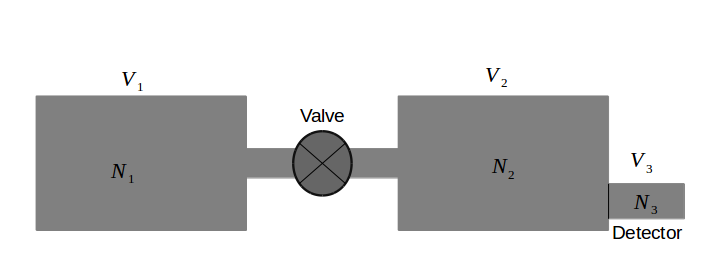
\includegraphics[width=0.9\textwidth]{volume_schematic.png}
  \caption{Schematic drawing of a simple UCN source. $V_1$ is the
    production volume with $N_1$ number of UCN, $V_2$ is the secondary
    volume where $N_2$ number of UCN exist, and $V_3$ is the detector
    with $N_3$ number of UCN. }
  \label{fig:volume_schematic}
\end{figure}

At $t = 0$, when the beam is on and the valve is closed, the number of UCN in
$V_1$ goes up, while the total number of UCN in $V_2$ and $V_3$ is
zero. This is described with 

\begin{equation}
  \label{eqn:dndt}
\frac{dN_1}{dt} = P - \frac{N_1}{\tau_1}~,
\end{equation}
where $P$ is the UCN production rate in the source, as describe in
Section~\ref{sec:UCN_production}, and $\tau_1$ is the UCN storage
lifetime in the source. After the beam is turned off, the valve is
opened, and UCN could travel to the volume $V_2$ and eventually volume
$V_3$. In our measurements, the valve is usually left open for 2
minutes. The UCN trade between $V_1$, $V_2$ and $V_3$ is described by
the differential Eqn.~\ref{eqn:alldndt}.

\begin{equation}
  \label{eqn:alldndt}
  \begin{aligned}
    \frac{dN_1}{dt} =&- \frac{N_1}{\tau_{c,1}} - \frac{N_1}{\tau_1} + \frac{N_2}{\tau_{c,2}}  \\
    \frac{dN_2}{dt} =& \frac{N_1}{\tau_{c,1}} - \frac{N_2}{\tau_{c,2}} - \frac{N_2}{\tau_2} - \frac{N_2}{\tau_{c,3}} \\
    \frac{dN_3}{dt} =& \frac{N_2}{\tau_{c,3}}~.
  \end{aligned}
\end{equation}


In these equations,$dN_1/dt$ shows the change in the UCN counts over
time in $V_1$, $dN_2/dt$ shows the change in the UCN
counts in $V_2$, and $dN_3/dt$ shows the
change in the UCN count in $V_3$, after the valve is opened. Each term
in the right side of the equations is described below.

In the first equation, the total number of UCN in $V_1$ depends on
three factors: the UCN that get into $V_2$ with the rate
$N_1/\tau_{c,1}$, the UCN that is lost with the storage lifetime
$\tau_1$ with the rate rate $N_1/\tau_{1}$, and the UCN that bounce
back from $V_2$ to $V_1$ with the rate $N_2/\tau_{c,2}$. Here
$1/\tau_{c,1}$ is the probability of UCN crossing from volume $V_1$ to
volume $V_2$, and $1/\tau_{c,2}$ is the probability of UCN cross from
volume $V_2$ back to volume $V_1$.


In the second equation for $V_2$, some UCN cross from $V_1$ to $V_2$
with the rate $N_1/\tau_{c,1}$, some get lost with the rate
$N_2/\tau_2$, some cross the gate valve and go back to $V_1$ with the
rate$N_2/\tau_{c,2}$, and some get to the detector with the rate
$N_2/\tau_{c,3}$. Here $1/\tau_{c,3}$ is the probabiliy of UCN
crossing from volume $V_2$ to volume $V_3$ and $1/\tau_2$ is the loss
probability of UCN in volume $V_2$.



In the third equation, the rate of the UCN detection $dN_3/dt$ is the
rate of UCN crossing from volume $V_2$ to volume $V_3$ as
$N_2/\tau_{c,3}$. In principle, solving these equations could give an
estimate of the number of UCN in each volume.

A 3D drawing of the experimental setup is shown in
Fig.~\ref{fig:Source_all}. In this case, $V_1$ is the UCN source
bottle, and the horizontal section of the UCN guide before the UCN gate
valve, and $V_2$ and $V_3$ are the volumes after the UCN valve and the
detector volume respectively.


The process of UCN production described above is refered to the UCN
production in the ``batch mode'', since the UCN is accumulated in the
source while the UCN valve is left closed. Here the target is
irradiated, and the UCN are produced in the source. After the
irradiation stops, the UCN valve is opened, and UCN could bounce of
the guide walls and reach the detector volume. In our standard UCN
production measurements, the applied beam current is 1~$\mu$A, and the
target is irradiated for 60~s. One cycle of measurement is shown in
Fig.~\ref{fig:UCNRate}. The UCN valve is typically left open for 2
minutes. The end of a UCN cycle is defined by the UCN valve close
time. Once the UCN valve is closed, a new cycle of measurement starts.


\begin{figure}[h!]
  \centering
  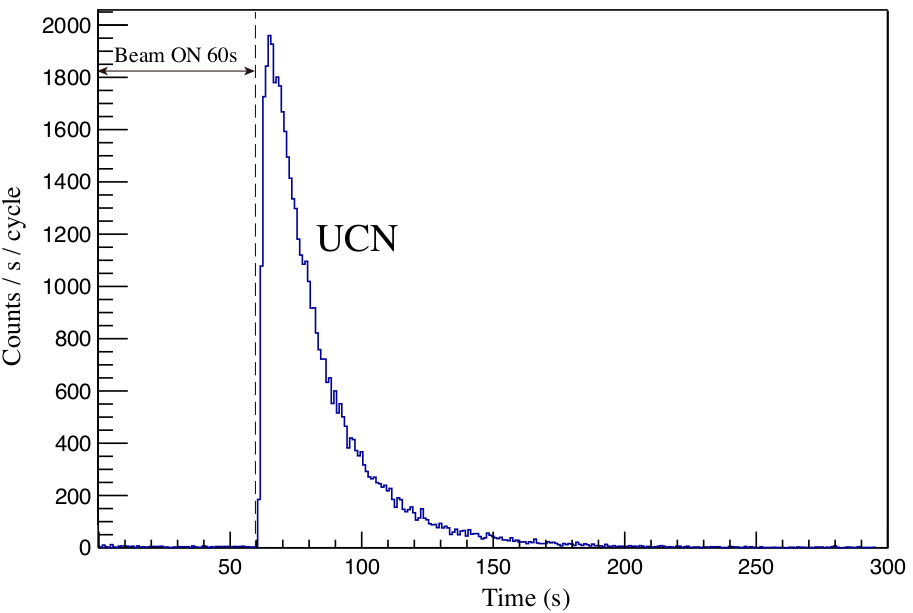
\includegraphics[width=0.8\textwidth]{UCNRate.png}
  \caption{The figure shows the UCN rate at 60~s irradiation time, and
    1~$\mu$A beam current. In this case, the UCN gate valve is opened
    immediately after the end of target irradiation. At this time, the
    UCN rate reaches the peak of about 2000 UCN/s. The UCN rate decays
    down to the background level. The valve is left open for 120~s. }
  \label{fig:UCNRate}
\end{figure}


Another possible mode of operation is when we leave the UCN valve open
while irradiating the target. This is called the ``steady-state
mode'' where we have a constant stream of UCN to the main
detector~(see Section~\ref{sec:steadystate}).

The following sections are focused on the result of the UCN yield
optimization, the UCN storage lifetime measurements, UCN production in
the steady-state mode and the comparison of those measurements with
simulations.


\section {Data Quality Checks}
During the 2017 experimental run, we performed about 35
experiments. For most of these experiments we used the $^6\mathrm{Li}$
glass based scintillator detector that was described in
Section~\ref{sec:Li6detector}. The data that is described is this
chapter is all acquired with the $^6\mathrm{Li}$ detector.  To check
the reliablitiy of this data we performed some data quality checks
that are reported here.

%The main detector for most of the experiments is the $^6\mathrm{Li}$
%glass based scintillator detector described in
%Section~\ref{sec:Li6detector}. Before using the collected data to
%extract the desired information, it is critical to make sure that the
%detector was working as expected, and that the data is reliable. Here
%some data quality checks are reported.


The PSD versus $Q_L$ distribution from a UCN run is shown in
Fig.~\ref{fig:psd_vs_ql} for all the PMTs combined. This is the most
useful way of separating the signal and background.
% The graph is for run 541
\begin{figure}[h!]
  \centering
  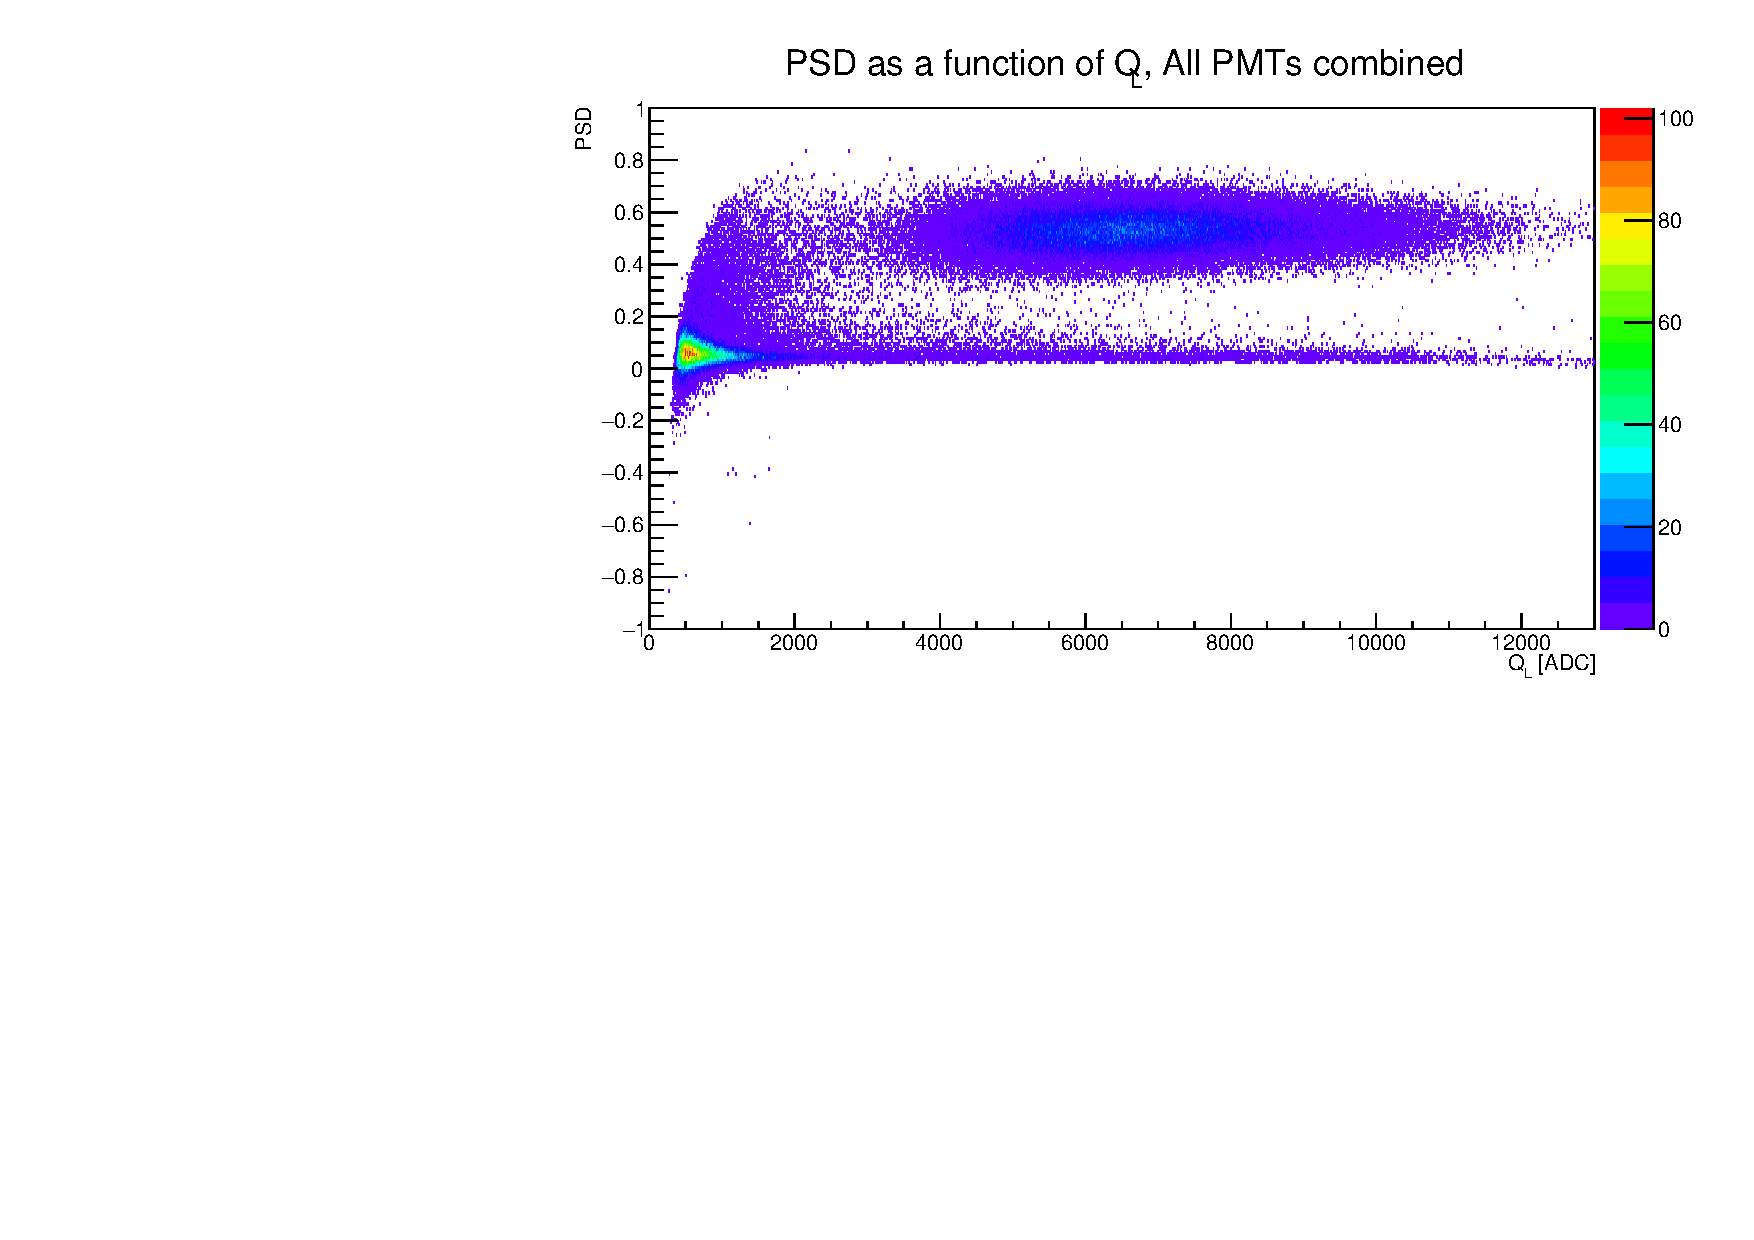
\includegraphics[width=0.9\textwidth]{PSD_vs_QL.pdf}
  \caption{PSD versus $Q_L$ for all of the PMTs for a standard
    1~$\mu$A proton beam current and 60~s target irradiation time }
  \label{fig:psd_vs_ql}
\end{figure}

Here the UCN spectrum has an energy range of 3000 to 12000 $Q_L$ as
expected, and a median PSD value of 0.5. The events at PSD~$\sim 0$
represent the $\gamma$-rays in the lightguides. To get the actual UCN
counts, a PSD cut at 0.3 and a $Q_L$ cut at 2000 were applied.  Those
cuts were confirmed with Monte-Carlo simulations to have an acceptance
of 99\% or higher. This ensures that only the UCN events are counted
which are represented by the central oval-shaped region. Out of all 9
channels, the centeral channel counts the most number of UCN events,
while the corner channels receive the least as expected~(see
Fig.~\ref{fig:channelcounts}).

\begin{figure}[h!]
  \centering
  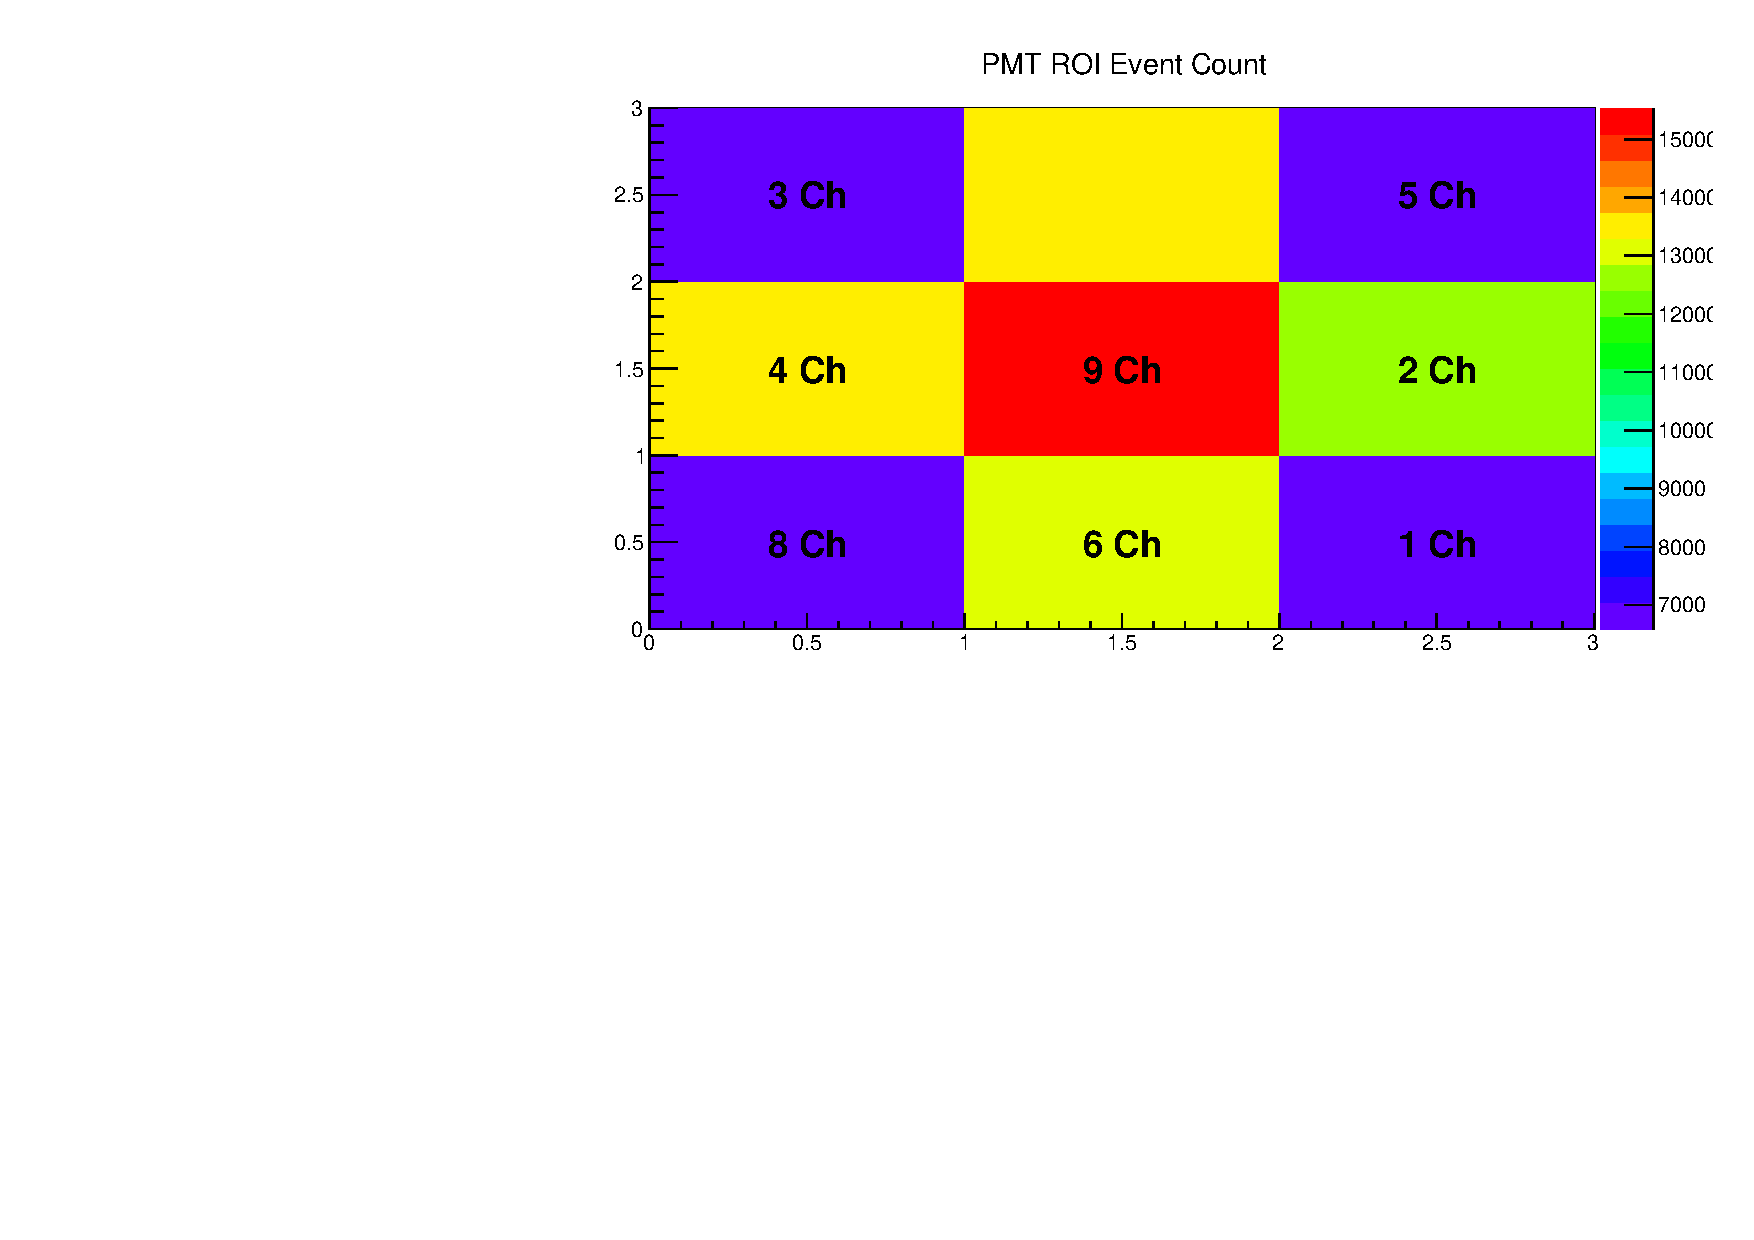
\includegraphics[width=0.9\textwidth]{channelcounts.pdf}
  \caption{Number of UCN events for each channel. The total number of
    UCN events decrease as we move towards the corner channels.  }
  \label{fig:channelcounts}
\end{figure}


The effect of the detector on the UCN counts could be categorized in
three groups: Deadtime, Crosstalk and Pileup. Deadtime is the minimum
time difference between two subsequent UCN events in the same PMT,
which might give rise to loss in the UCN counts. Crosstalk is the
multiple trigger events in neighboring PMTs originated from the same
UCN events. This effect might increase the possiblitiy of
overestimating the total UCN counts. Pileup is the combination of
multiple events into a single event. It includes UCN-UCN,
UCN-$\gamma$, $\gamma$-UCN and $\gamma$-$\gamma$ pileups. The true
number of UCN counts is estimated by
\begin{equation}
  \label{eqn:trueUCN}
  N^{\mathrm{True}}_{\mathrm{UCN}} = \left [ N^{\mathrm{raw}}_{\mathrm{UCN}} \cdot \left( 1 + \alpha_{pl} + \alpha_{ct}\right) \right] \cdot A_{box}~,
\end{equation}
where $\alpha_{pl}$ is the estimated pileup coefficient from data and
independant calculations assuming Poisson statistics, $\alpha_{ct}$ is
the estimated time-coincidence analysis on data, and $A_{box}$ is the
UCN box efficiency estimated using Monte-Carlo simulations. Based on
our Monte-Carlo simulations, the $\gamma$-UCN and UCN-$\gamma$ pileups
are not a concern for UCN counting. In addition, $\gamma$-$\gamma$
pileup does not leak into the UCN box.

The result of such analyses showed the UCN box acceptance is at
99.7 $\pm$ 0.1~\%. The UCN-UCN pileup at 1~$\mu$A beam current and 60~s
irradiation of the target was measured to be at 0.075~Hz or has and
effect of less than 1~\%. The analysis indicated that cross-talk has a
negligible effect on the operating rates and deadtime affects the
rates by less than 2~\%.


%% I should think about adding MC simulations by Pietro, maybe???
%%

\section{UCN Count Measurements \label{UCNCounts}}

The total number of produced UCN in the vertical source, $N$, at a
certain time t$_i$, when the UCN valve is closed is the integration of
Eqn.~\ref{eqn:dndt}
\begin{equation}
  \label{eq:totalUCN}
  N = P \tau_1\left[ 1- \exp \left(\frac{t_i }{ \tau_1}\right) \right]~,
\end{equation}
where the UCN storage lifetime $\tau_1$ is given by

\begin{equation}
  \label{eqn:tau1}
  \frac{1}{\tau_1} = \frac{ f_1}{\tau_\mathrm{He}} + \frac{1-f_1}{\tau_\mathrm{vapour}}+\frac{1}{\tau_\mathrm{wall,1}} + \frac{1}{\tau_\beta}~.
\end{equation}
The storage lifetime consists of four terms: the loss rate in the
superfluid helium $ f_1\tau_\mathrm{He}^{-1}$, the loss rate in the
helium vapour $(1-f_1)\tau_\mathrm{vapour}^{-1}$, the loss rate in the
UCN guide walls $\tau_\mathrm{wall,1}^{-1}$, and the neutron $\beta$
decay $\tau_\beta^{-1}$. The volume in which the UCN are produced
includes the UCN bottle, as well as the horizontal guide section
before the UCN valve~(see Fig.~\ref{fig:Source_all}). This volume is
not fully filled with the superfluid helium. As a result, $ f_1$ is
the probablity of UCN being in the superfluid helium while the UCN
valve is closed. After the valve is opened, the total UCN lifetime is

\begin{equation}
  \label{eqn:tau2}
  \frac{1}{\tau_2} = \frac{ f_2}{\tau_\mathrm{He}} + \frac{1-f_2}{\tau_\mathrm{vapour}}+ \frac{1}{\tau_\mathrm{wall,2}}+\frac{1}{\tau_d} + \frac{1}{\tau_\beta}~,
\end{equation}
where $f_2$ is the probability of UCN being in the superfluid helium,
${\tau_\mathrm{wall,2}}^{-1}$ is the UCN guide loss rate in the case
where the valve is open and the target irradiation is stopped, and
$\tau_d^{-1}$ is the loss rate in the
detector. Fig.~\ref{fig:UCNRate_with_lines} shows three measurement
cycles at 1~$\mu$A beam current, and 60~s irradiation time with zero
second delay time between the end of the target irradiation and
opening the UCN valve~(here sometimes this is referred to as the cycle
delay time or valve open delay time). The dashed lines indicate the
start of the target irradiation for a cycle, the dotted lines show the
end of the target irradiation, which in this case is the same as the
UCN valve open time. The solid lines shows the valve close time.


\begin{figure}[h!]
  \centering
  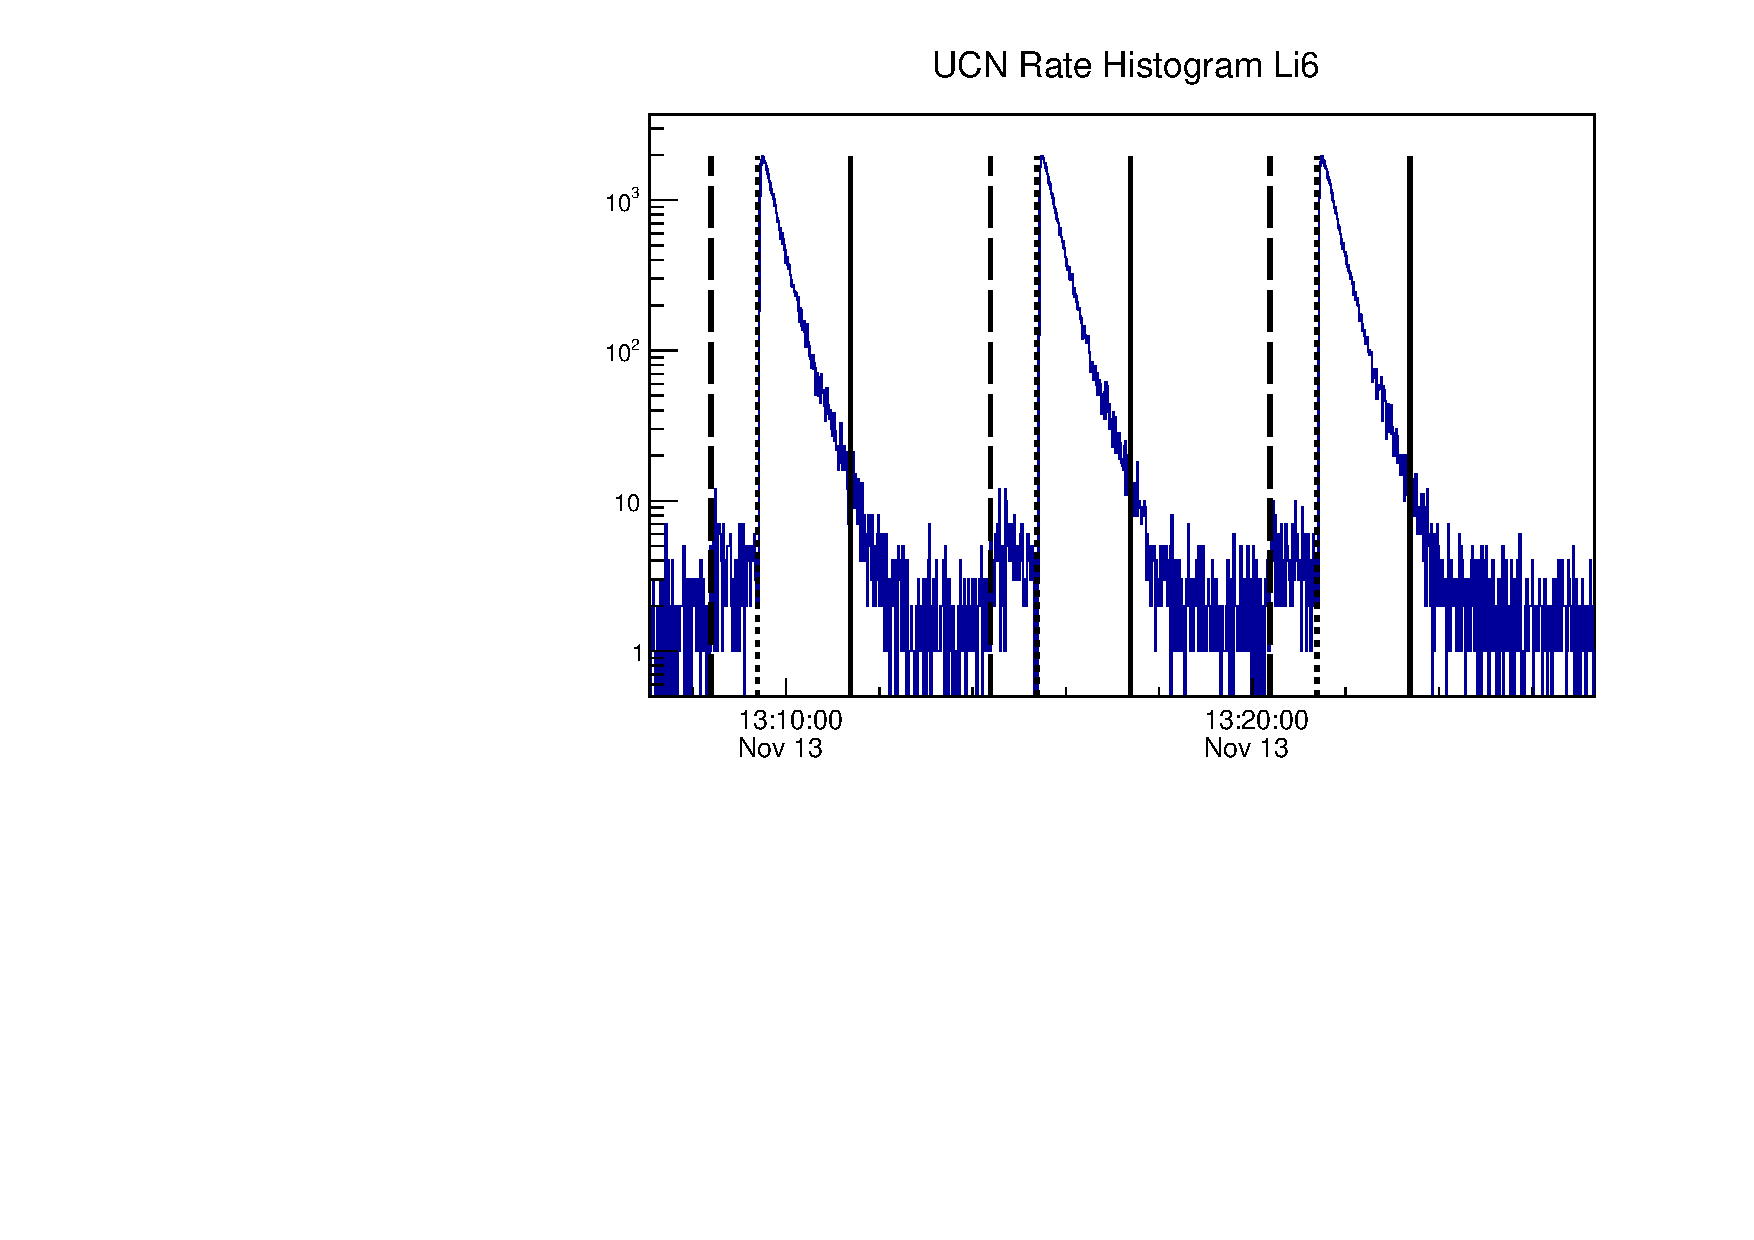
\includegraphics[width=1.0\textwidth]{UCNRate_with_lines_logy.pdf}
  \caption{Three measurement cycles for 1~$\mu$A beam current, 60~s
    irradiation time, and 0~s valve open delay time. The dashed lines
    show the start of the target irradiation, the dotted lines show
    the end of the irradiation and the valve open time for each cycle
    and the solid lines show the end of a cycle, which is the valve
    close time.}
  \label{fig:UCNRate_with_lines}
\end{figure}

The total UCN counts are given by the integration of all the UCN
events for the duration of the valve open time. However, this method
of counting includes the measured background UCN as well. To subtract
the background counts from the actual UCN counts, the UCN background
rate is calculated before the start of the irradiation of that
particular cycle. This rate is then multiplied by the valve open
duration, which then gives an estimate of the total background UCN
counts. The background rate is typically less than 5~UCN/s. The
subtraction of the latter from the total UCN counts gives the actual
number of UCN that are produced by the isopure helium converter, and
detected by the detector. At low and moderate UCN counts, the
statistical uncertainty is available by taking the square root of the
number of measured events, as follows conveniently from Poisson
statistics~\cite{pomme2015uncertainty}.
%%%%%%%%%%
\subsection{UCN Yield Versus Proton Beam Current}
The UCN yield at different proton beam currents is also
studied. Fig.~\ref{fig:counts_vs_beam} shows the total UCN counts
versus the applied proton beam current in $\mu$A at 60~s irradiation
time. The background UCN is subtracted off from the detected UCN
counts as explained earlier. The error bar on the UCN counts is
calculated as $\sqrt{N}$. At lower beam currents, the total UCN counts
increase linearly with the proton beam current. The dashed line shows
the extrapolation to higher beam currents in an ideal case. However,
at higher beam currents, the total UCN counts deacreses due to an
increase in the heat load on the isopure superfluid helium, and
therefore, its temperature. Theoretically, the upscattering rate in
the superfluid helium is proportional to its temperature as $T^7$~(see
Section~\ref{sec:upscattering}). This has been confirmed by performing
PENTrack simulations and comparing the result to the acquired
data~(see Section~\ref{sec:pentrack}).



\begin{figure}[h!]
  \centering
  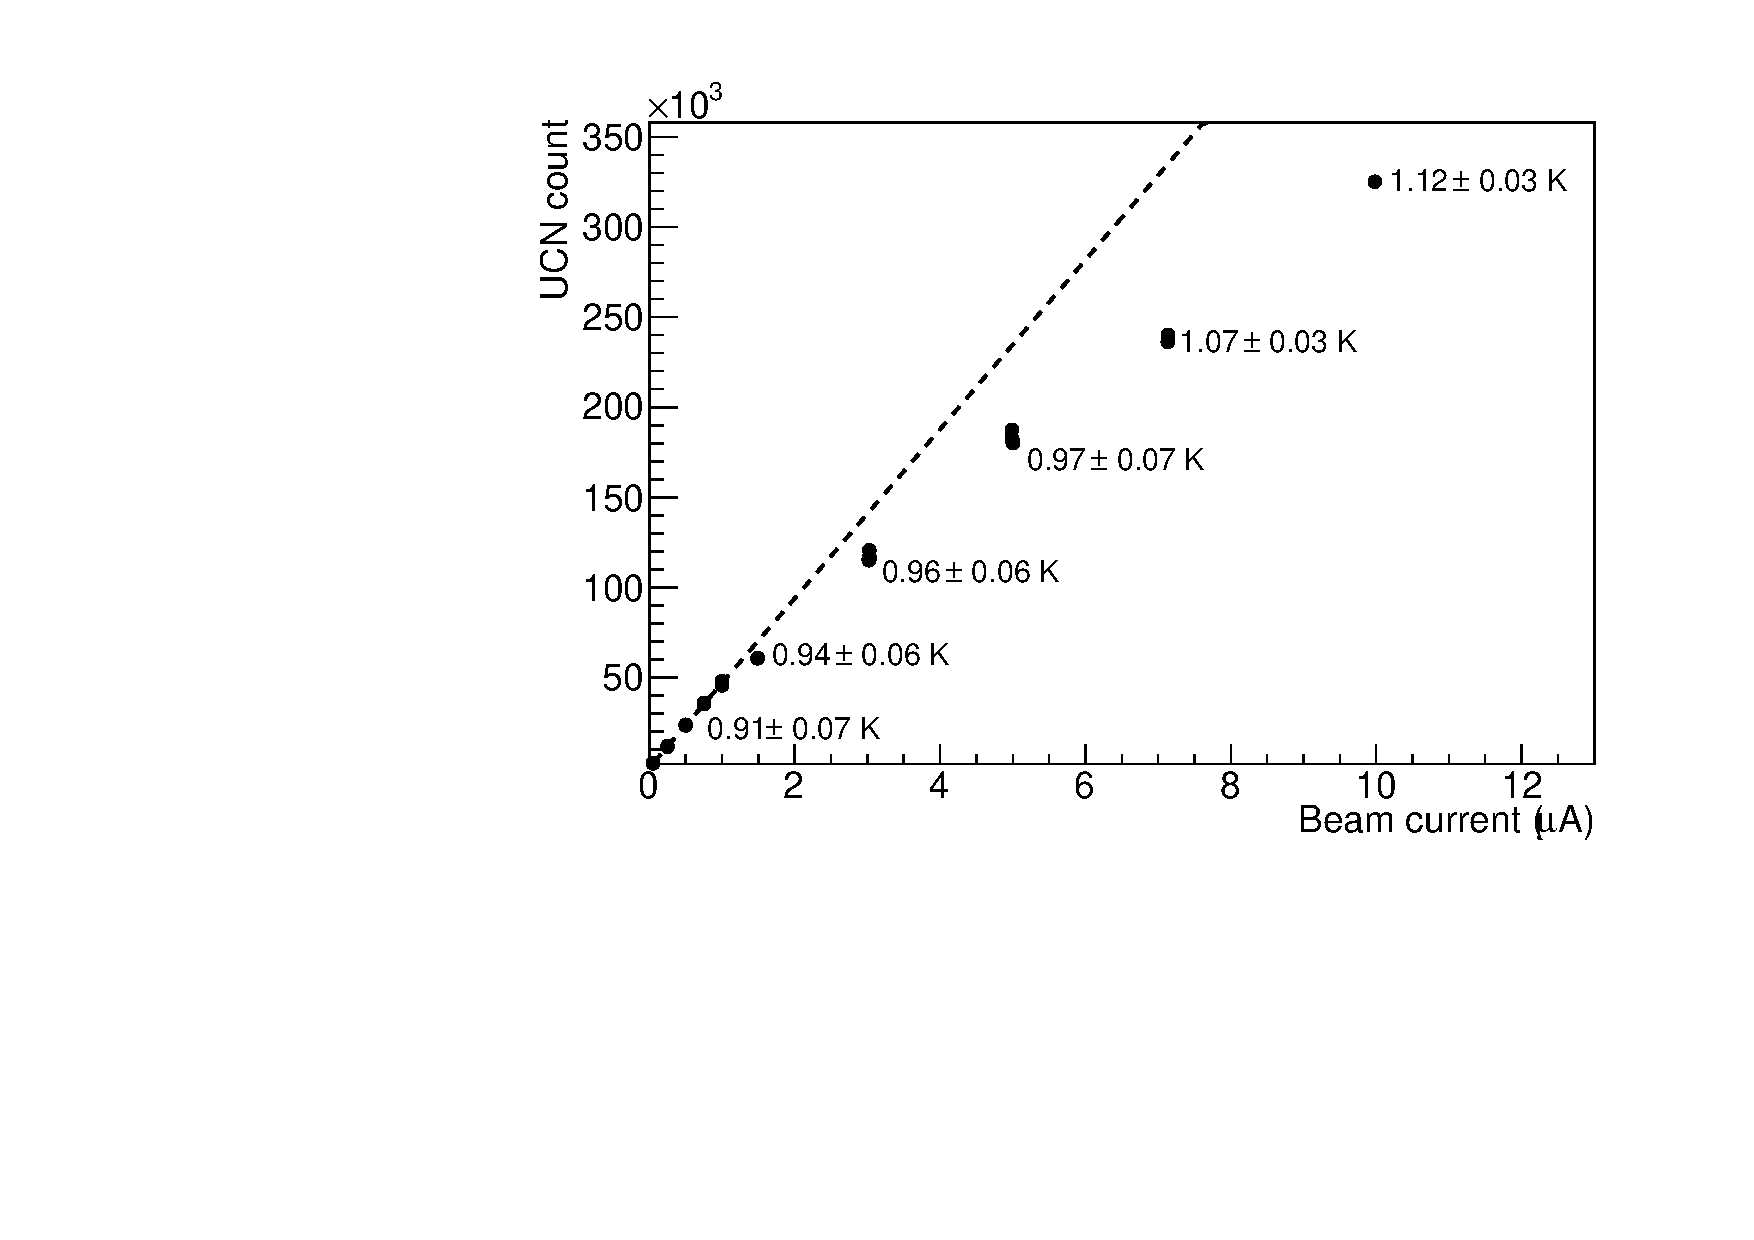
\includegraphics[width=0.8\textwidth]{UCNCounts_vs_Beam.pdf}
  \caption{The total UCN counts versus the applied proton beam
    current. The labelas show the full range of the superfluid helium
    temperature for that measurement. The dashed line is the fit to
    the UCN counts at low beam currents.}
  \label{fig:counts_vs_beam}
\end{figure}


The labels in the graph show the full range of the isopure helium
temperatures during the measurement cycle. Four temperature sensors
were used to measure the superfluid helium temperature with the
following names in our EPICS system: TS11, TS12, TS14 and TS16. The
location of these sensors are shown in Fig.~\ref{fig:TSs}. The
temperature sensor TS11 is located at the UCN heat exchanger bottom,
the temperature sensor TS14 is located at the UCN heat exchanger top,
the temperature sensor TS12 is located at the UCN double tube bottom,
and the temperature sensor TS16 is located at the UCN double tube
top. At low temperatures around 0.8~K, these temperature sensors show
a maximum of 0.1~K discrepancy with TS16 showing the highest value,
and TS12 showing the lowest value.


\begin{figure}[h!]
  \centering
  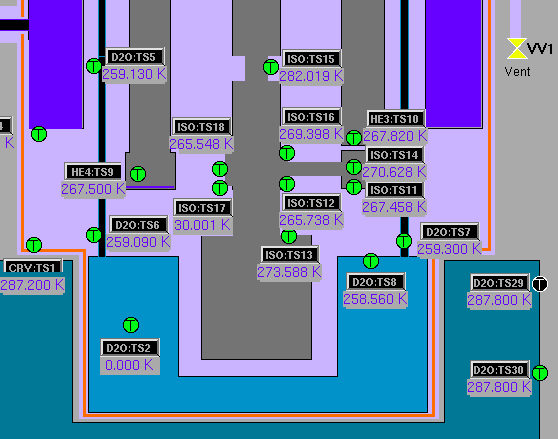
\includegraphics[width=0.8\textwidth]{TSs.png}
  \caption{Zoomed in screenshot of the EPICS temperature monitoring
    screen~\ref{fig:epics}. TS11 is located at the UCN heat exchanger
    bottom, TS12 is located at the UCN double tube bottom, TS14 is
    located at the heat exchanger double tube top and TS16 is located
    at the UCN double tube top. For further information about the
    source schematic see Section~\ref{sec:vertical_source}}
  \label{fig:TSs}
\end{figure}

In summary, at lower beam currents, because of the low heat load on
the superfliud helium, its temperature change is not significant, and
it gives rise to a linear increase in the UCN counts versus at various
applied proton beam current. However, at higher proton beam currents,
the temperature of the superfluid increases due to a higher heat load,
and it gives rise to higher upscattering rate in the superfluid and
lower UCN counts.


\subsection{UCN Yield Versus Target Irradiation Times}
The total UCN counts is optimized by irradiating the target with
different proton beam currents at different irradiation times. The
result is shown in Fig.~\ref{fig:counts_vs_irrad}. In this graph, the
vertical axis shows the total number of UCN counts where the
background UCN are subtracted, and the horizontal axis shows the
target irradiation times in seconds. Each marker represents a proton
beam current. The dashed line is an exponential fit to those data
points. The proton beam current and the extracted time constant from
the fit are shown in the Figure.

At higher beam currents, the saturation time constant decreases due to
the higher heat load and faster temperature increase in the superfluid
helium. At higher beam currents and longer irradiation times, the
total measured UCN counts are below the exponential extrapolation due
to the higher temperature and higher upscattering rate in the
superfluid helium.

\begin{figure}[h!]
  \centering
  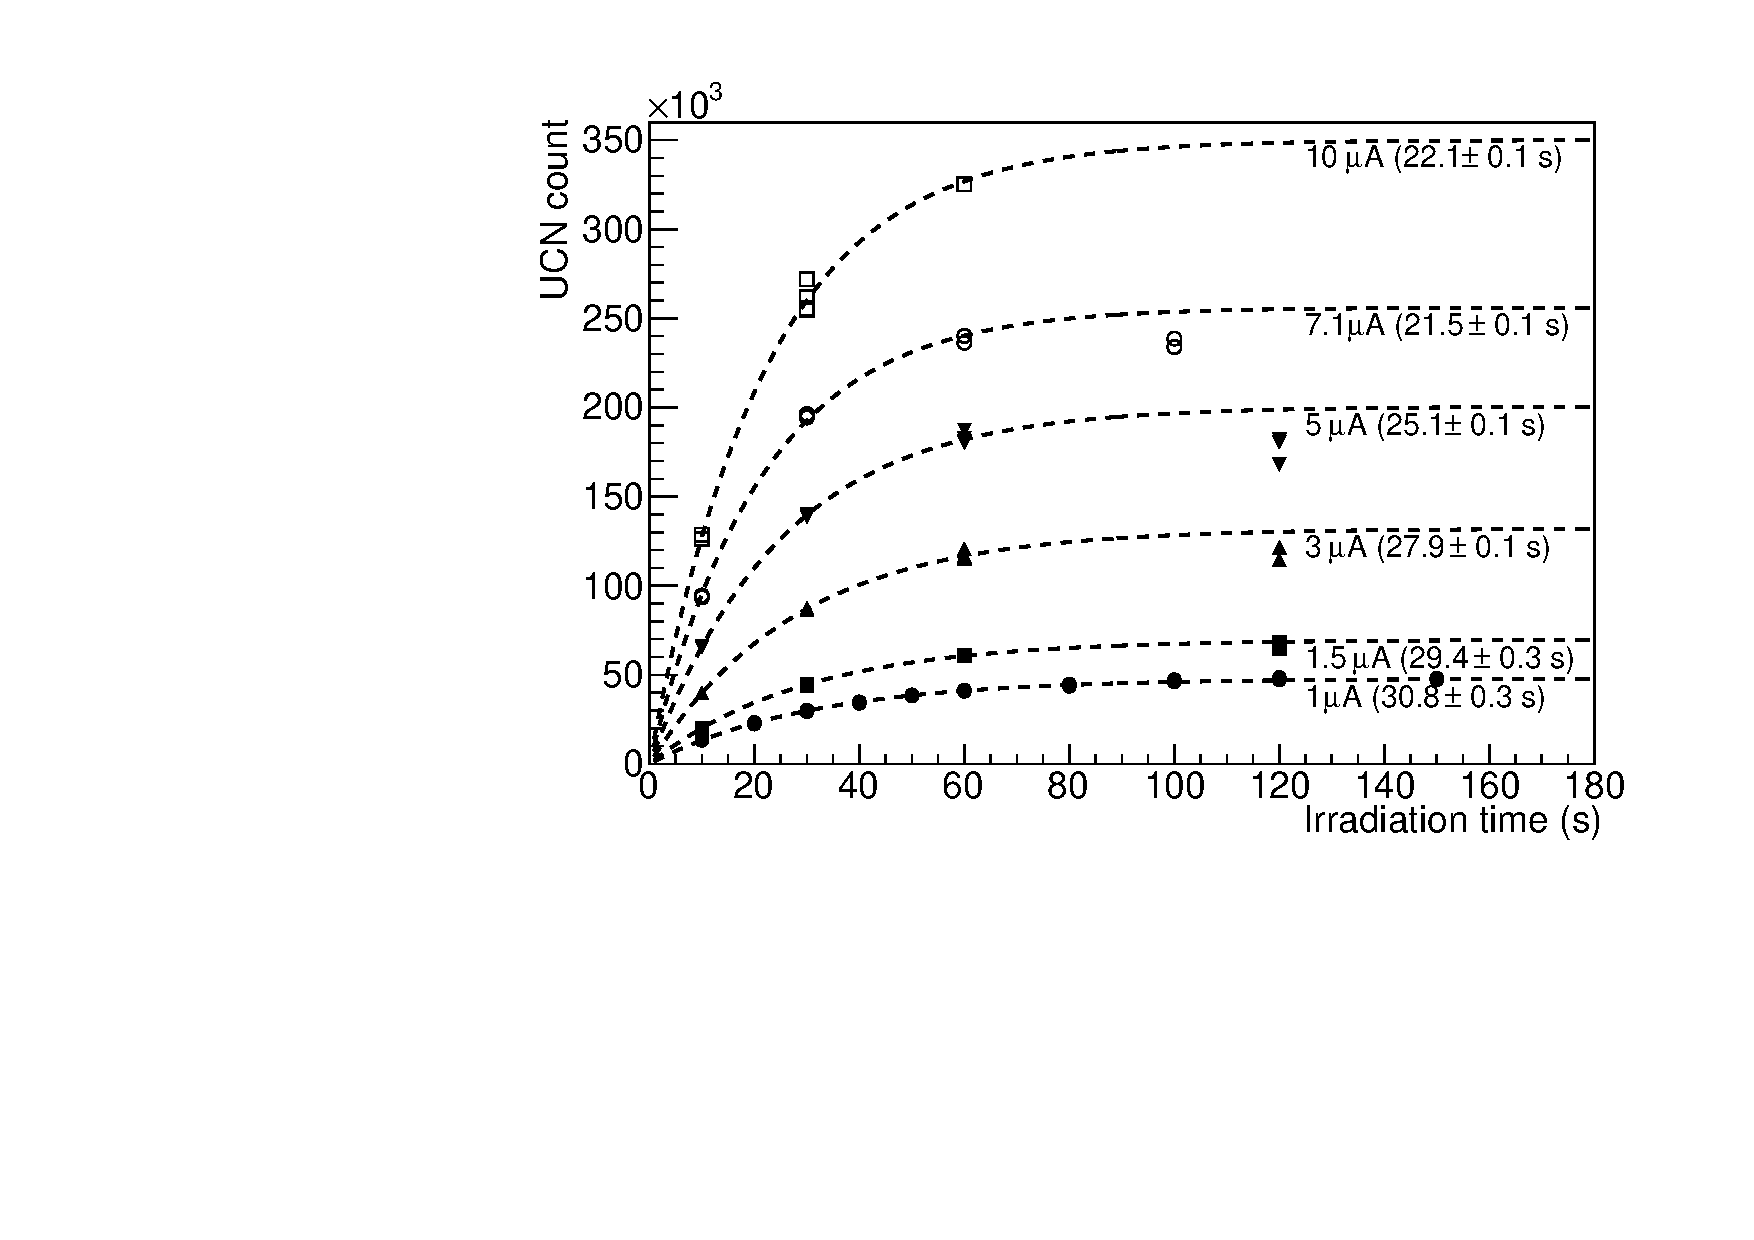
\includegraphics[width=0.8\textwidth]{UCNCounts_vs_irradTime.pdf}
  \caption{Number of UCN extracted from the source after irradiating
    the target for different times with different beam currents. The
    dashed lines extrapolate the data for irradiation times below 60~s
    using exponential saturation curves. The labels show the
    saturation time constant for each beam current. }
  \label{fig:counts_vs_irrad}
\end{figure}


\subsection{UCN Yield Versus Isopure Helium Temperature}
The UCN counts were also measured at different superfluid helium
temperature~(see Fig.~\ref{fig:counts_vs_temp}). The vertical axis
shows the number of UCN counts, and the horizontal axis shows the
temperature of the superfluid helium for all four temperature
sensors. The vertical error bars are $\sqrt{N}$, and the horizontal
error bars are calculated as $(T_{\mathrm{max}}-T_{\mathrm{min}})/2$
for each temperature sensor, where $T_{\mathrm{max}}$ is the maximum
value of the superfluid helium temperature reading by one temperature
sensor, and $T_{\mathrm{min}}$ is the minimum value read for the same
sensor.

\begin{figure}[h!]
  \centering
  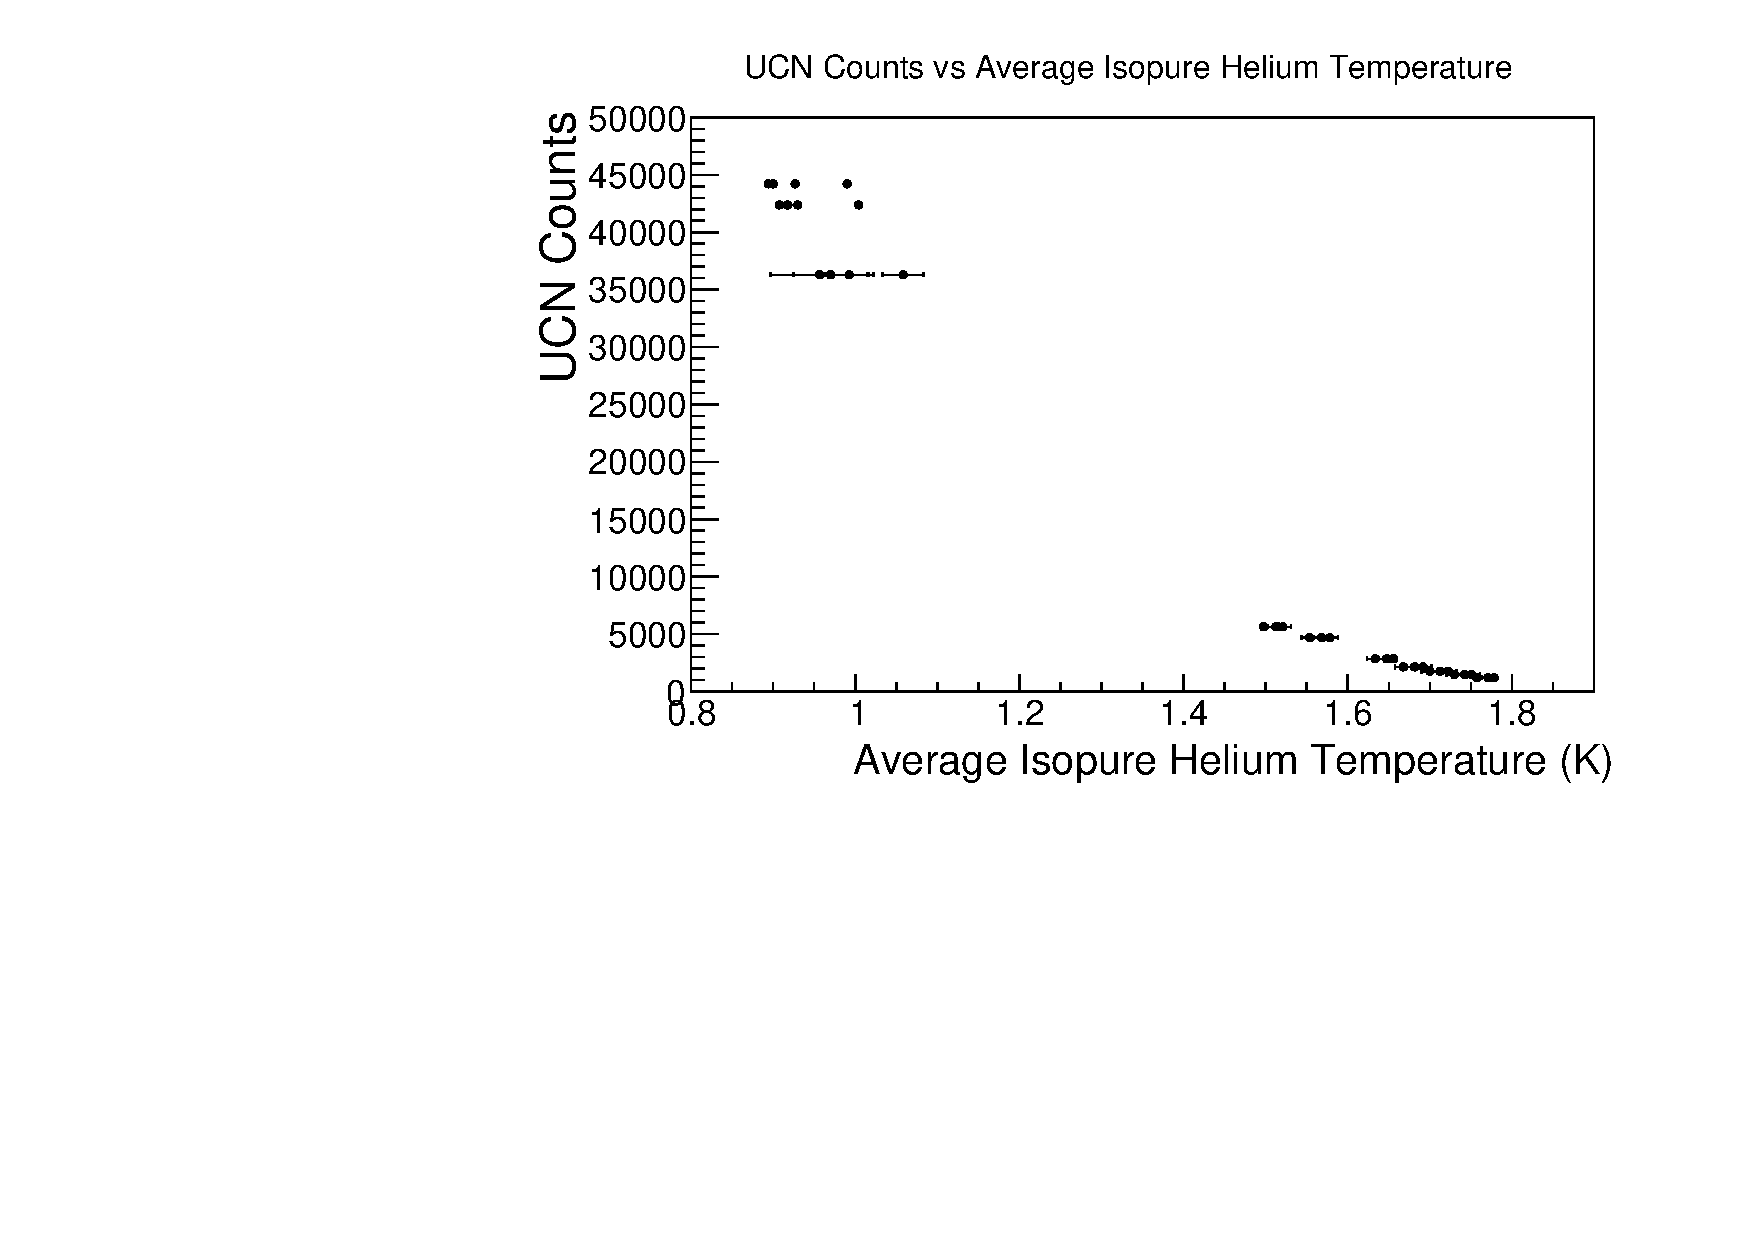
\includegraphics[width=0.9\textwidth]{counts_vs_temp.pdf}
  \caption{UCN yield versus the superfluid helium temperature. At a
    particular UCN counts, there are several values for the
    temperature of the superfluid helium. This is due to the
    discrepancy in the temperature sensor readings as described in the
    text.}
  \label{fig:counts_vs_temp}
\end{figure}

As the temperature of the superfluid helium increases, the
number of UCN counts in the detector decreases as expected. This is
mainly due to the high UCN upscattering rate in the superfluid helium
at higher temperatures.


\subsection{Steady-state UCN Production\label{sec:steadystate}}

The result shown so far are achieved in the batch mode of
operation. In addition to such measurements, the UCN rate was also
measured at different beam currents in the steady-state mode of
operation. In these measurements, the UCN valve was left open, and the
target was irradiated for about 10~min. A typicall UCN rate graph for
0.3~$\mu$A beam current and 10~min target irradiation time is shown in
Fig.~\ref{fig:UCNRate_steadystate}.


\begin{figure}[h!]
  \centering
  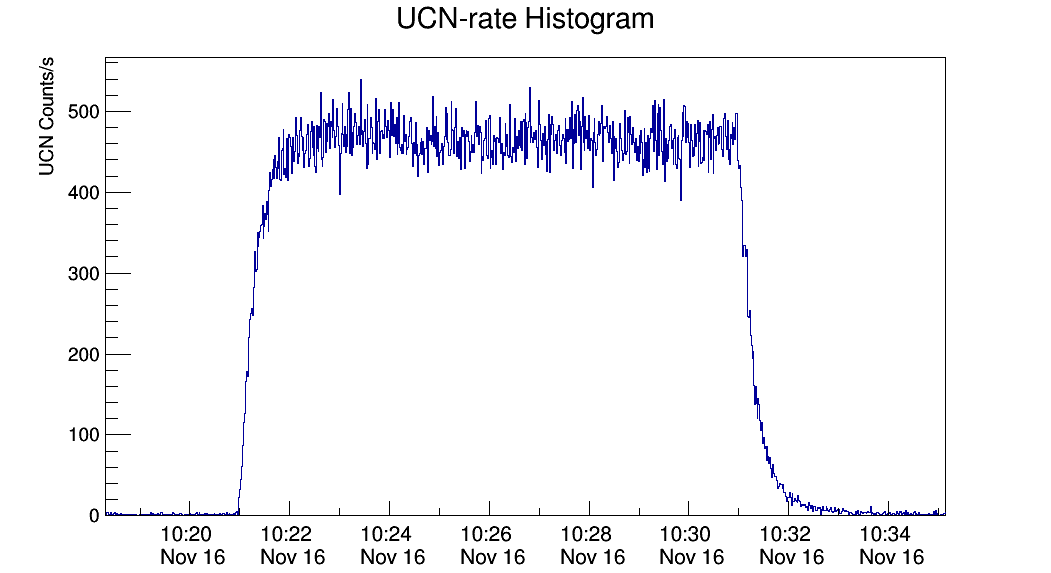
\includegraphics[width=0.9\textwidth]{steadystate_point3muA.png}
  \caption{UCN rate at the steady-state production mode with 0.3~$\mu$A proton beam
    current. The UCN rate reaches a constant value of 450 UCN counts/s.}
  \label{fig:UCNRate_steadystate}
\end{figure}

At lower beam currents such as 0.3~$\mu$A, the UCN rate remains
constant throughout the whole target irradiation time as shown in
Fig.~\ref{fig:UCNRate_steadystate}. An example of a steady-state UCN
production at 3~$\mu$A is shown in
Fig.~\ref{fig:UCNRate_steadystate_highbeam}. Since the proton beam
current is high, the UCN rate does not remain constant. Here the
maximum UCN rate is observed near the start of the target
irradiation. As the target irradiation continues, the heat load on the
cryostat increases the temperature, and the upscattering rate in the
superfluid helium. As a result, the UCN rate decreases. The change in
the temperature is shown in Fig.~\ref{fig:UCNRate_temp}. Throughout
the target irradiation time, the temperature of the superfluid helium
increases. Once the irradiation stops, the temperature starts to
decrease.


\begin{figure}[h!]
  \centering
  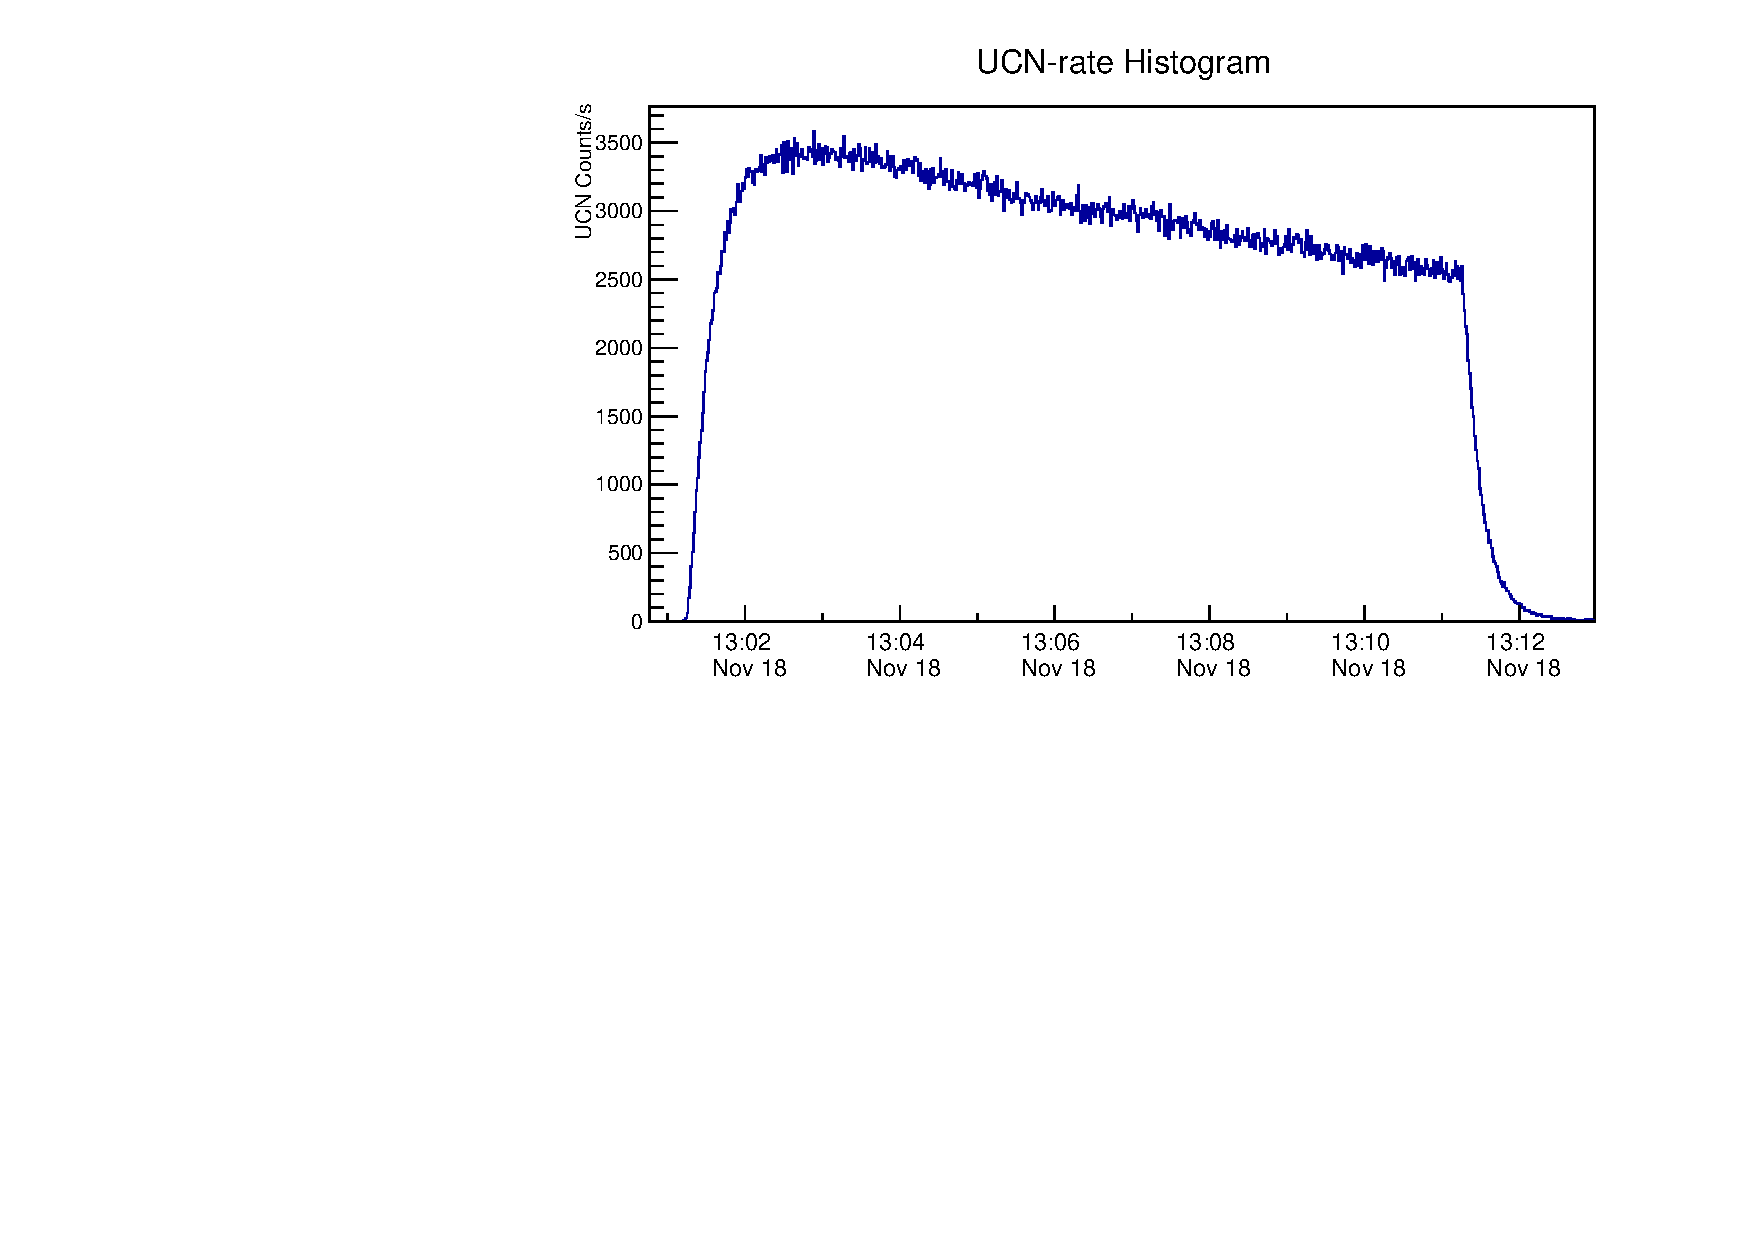
\includegraphics[width=0.9\textwidth]{654_UCNRate.pdf}
  \caption{The UCN rate at 3~$\mu$A beam current at 10~min irradiation
    time at the steady-state mode of operation. The UCN valve is left
    open throughout the measurement cycle. Quickly after the start of
    the target irradiation the UCN rate in the detector goes up. The
    target irradiation creates a heatload on the cryostat and the
    superfluid helium. This gives rise to a slow temperature increase
    in the source. As a result, the UCN rate goes down due to the
    higher upscattering rate.  }
  \label{fig:UCNRate_steadystate_highbeam}
\end{figure}

\begin{figure}[h!]
  \centering
  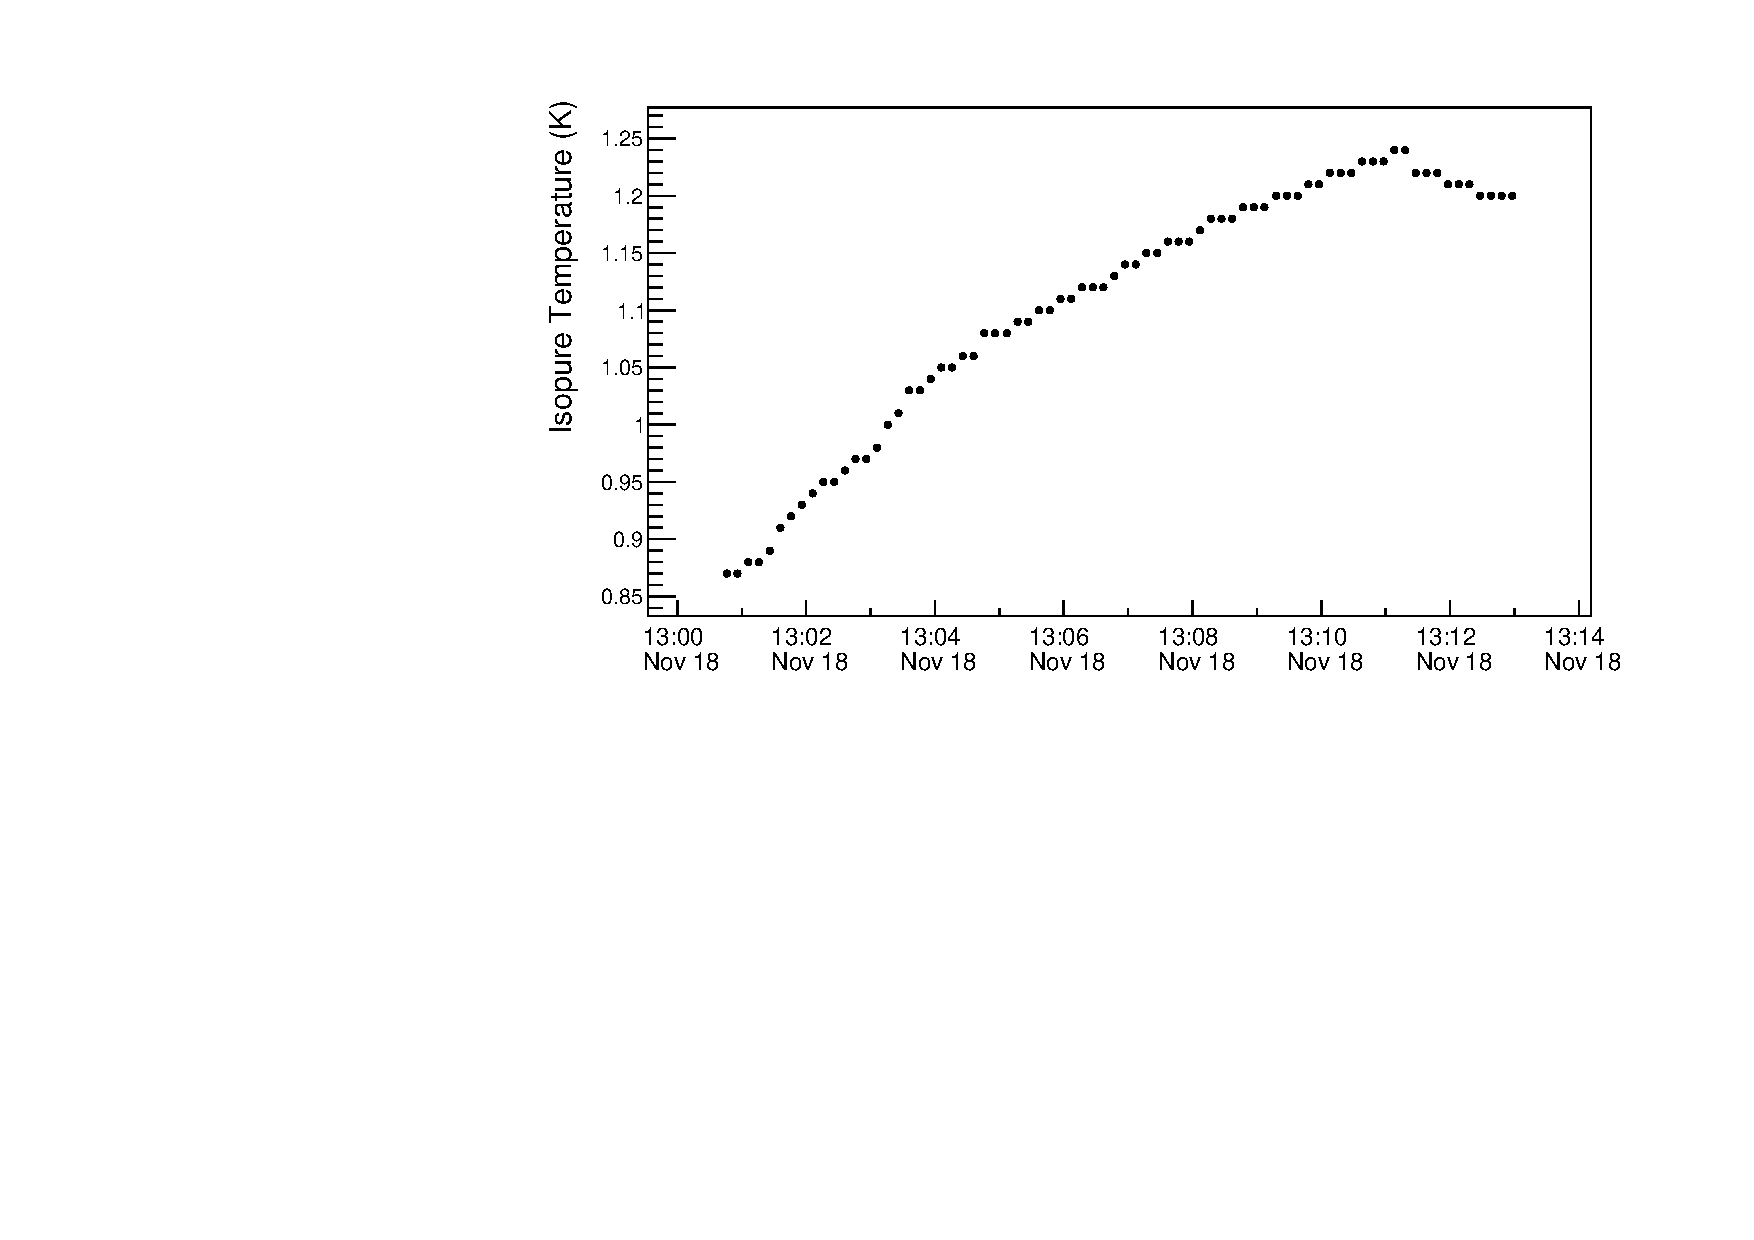
\includegraphics[width=0.9\textwidth]{UCNRate_temp.pdf}
  \caption{ The temperature of the superfluid helium~(TS12) for the
    steady state mode of operation at 3~$\mu$A beam current and 10~min
    target irradiation. After the irradiation stops, the temperature
    starts to decrease. }
  \label{fig:UCNRate_temp}
\end{figure}


The steady-state UCN rate measurements were conducted at different
proton beam currents, leading to different temperature changes for all
temperature sensors. The result of all those measurements and
comparison to simulations are discussed in Section~\ref{sec:pentrack}.


%are shown in
%Fig.~\ref{fig:rate_vs_temp}. Here the vertical axis is the measured
%UCN rate normalized to the proton beam current and the horizontal axis
%is the temperature of the superfluid helium for all temperature
%sensors.


%\begin{figure}[h!]
%  \centering
%  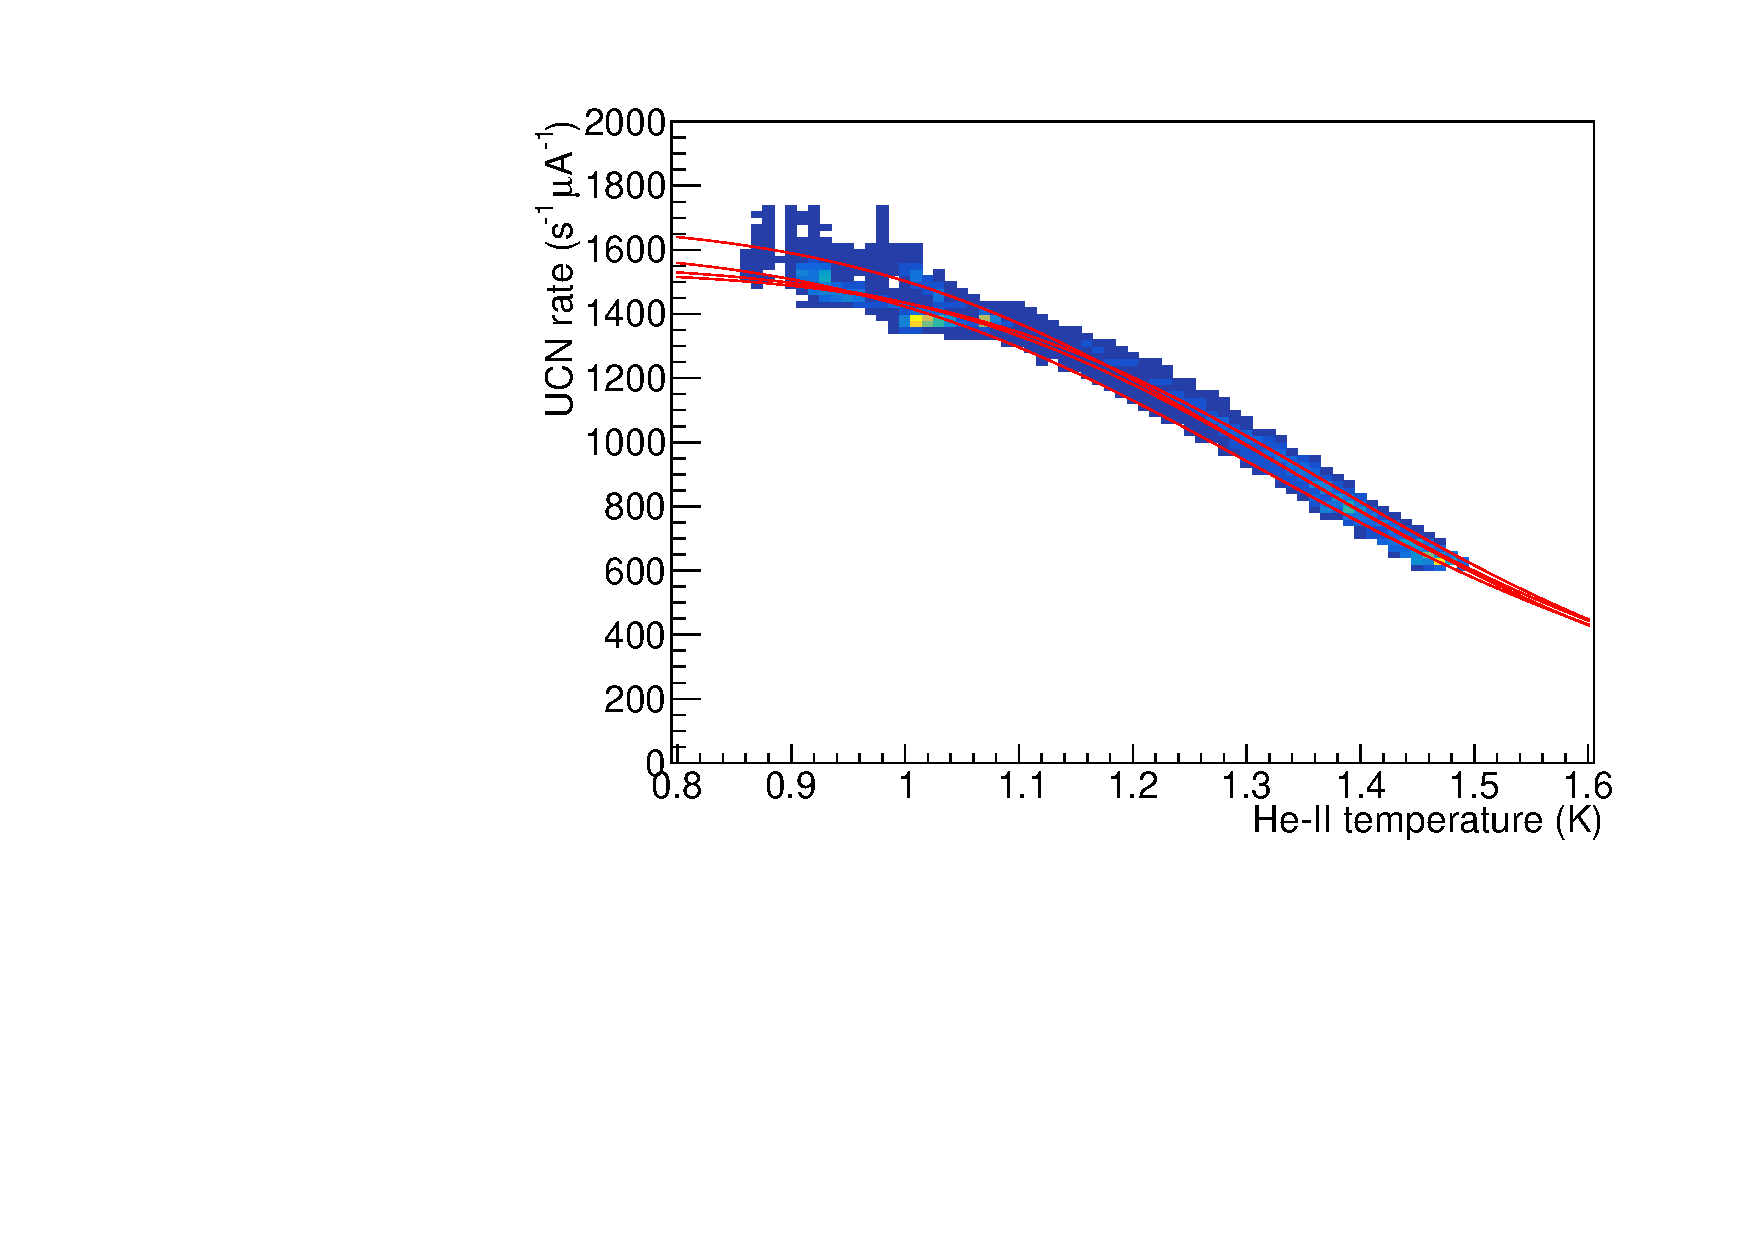
\includegraphics[width=0.7\textwidth]{rate_vs_temp.pdf}
%  \caption{Histogram of measured UCN rates and temperatures from all
%    four temperature sensors while the target is continuously
%    irradiated with the UCN valve open. The four solid lines are fits
%    of equation~\ref{eq:steadystaterate} to the data for each individual temperature
%    sensor.}
%  \label{fig:rate_vs_temp}
%\end{figure}


%The rate of the detected UCN is given by

%\begin{equation}
%  \label{eqn:rate}
%  R = \frac{P \tau_3}{\tau_d} = \frac{P \tau_d^{-1}}{\tau_\mathrm{wall,2}^{-1} + \tau_d^{-1} + f_\mathrm{He,3}\tau_\mathrm{He}^{-1}}
%\end{equation}
%where $\tau_d^{-1}$ is the loss rate in the detector,
%${\tau_\mathrm{wall,2}}^{-1}$ is the UCN guide wall loss and
%$\tau_\mathrm{He}^{-1}$ is the loss rate in the superfluid helium.
%Assuming $\tau_\mathrm{He}^{-1} = B \left( T \right)^a$ the
%Eqn.~\ref{eqn:rate} could be written as

%\begin{equation}
%R(T) = \frac{c}{1 + b \left( \frac{T}{\SI{1}{\kelvin}} \right)^{a}}
%\label{eq:steadystaterate}
%\end{equation}
%where \large
%$b = \frac{f_{\mathrm{He,3}}B}{\tau^{-1}_{\mathrm{wall,2}}
%  +\tau^{-1}_d}$ \normalsize and \large
%$c = \frac{P\tau^{-1}_d}{\tau^{-1}_{\mathrm{wall,2}} +\tau^{-1}_d}$
%\normalsize.  Eqn.~\ref{eq:steadystaterate} can be used to fit the
%data shown in Fig.~\ref{fig:rate_vs_temp}.  Since the four temperature
%sensors in the superfluid helium deviate by up to \SI{0.1}{\kelvin},
%the rate for each temperature sensor is fitted individually (see
%table~\ref{tab:steadystateparams}). The exponent $a$ can be directly
%determined this way, giving
%\begin{equation}
%a = 7.02 \pm 0.02_\mathrm{stat.} \pm 0.53_\mathrm{syst.},
%\label{eq:a}
%\end{equation}
%which is in good agreement with the theoretical prediction of $a = 7$
%(see Sec.\ref{sec:upscattering}). Here the statistical error comes
%from the fit and the systematic error comes from the temperature
%difference from the sensors and their propagated error.


%The other parameters are
%\begin{align}
%\label{eq:b}
%  b =&  0.0995 \pm 0.0007_\mathrm{stat.} \pm 0.0298_\mathrm{syst.} \\
%  c =& (1610 \pm 1_\mathrm{stat.} \pm 75_\mathrm{syst.}) \, \si{\per\second}
%\end{align}

%\begin{table}[h!]
%  \centering
%  \begin{tabular}{|c|c|c|c|}
%    \hline
%      Temp. sensor & $a$ & $b$ & $c$ (\si{\per\second}) \\
%      \hline
%      TS11 & $7.55 \pm 0.03$ & $0.0697 \pm 0.0009$ & $1535 \pm 1$ \\
%      \hline
%      TS12 & $6.48 \pm 0.03$ & $0.1293 \pm 0.0016$ & $1606 \pm 2$ \\
%      \hline
%      TS14 & $7.34 \pm 0.03$ & $0.0832 \pm 0.0011$ & $1555 \pm 2$ \\
%      \hline
%      TS16 & $6.67 \pm 0.04$ & $0.1215 \pm 0.0019$ & $1685 \pm 3$ \\
%      \hline
%    \end{tabular}
%  \caption{Parameters determined by fitting equation
%    \ref{eq:steadystaterate} to the measured rates shown in
%    fig. \ref{fig:rate_vs_temp} for each individual temperature
%    sensor.}
%  \label{tab:steadystateparams}
%\end{table}



\subsection{UCN Yield Over the Experiment Period}

The total UCN counts for our standard measurements at 1~$\mu$A beam
current and 60~s irradiation time over the course of the experimental
run is shown in Fig.~\ref{fig:UCNCounts_time}. The graph shows an
overall decrease of about $\sim$~40\% over the course of the eighteen
days. The source volume is connected to a long UCN guide sealed with
an O-ring. It is expected that the rest gas to contaminate the source
every time the UCN valve is opened. This caused a decrease in the UCN
yield~(and storage lifetime as shown later in
Section~\ref{sec:storage_overall}) over the course of the
measurement. In addition, the changes in the UCN guide geometry in the
latter half of the run pottentially affected this drop.


\begin{figure}[h]
  \centering
  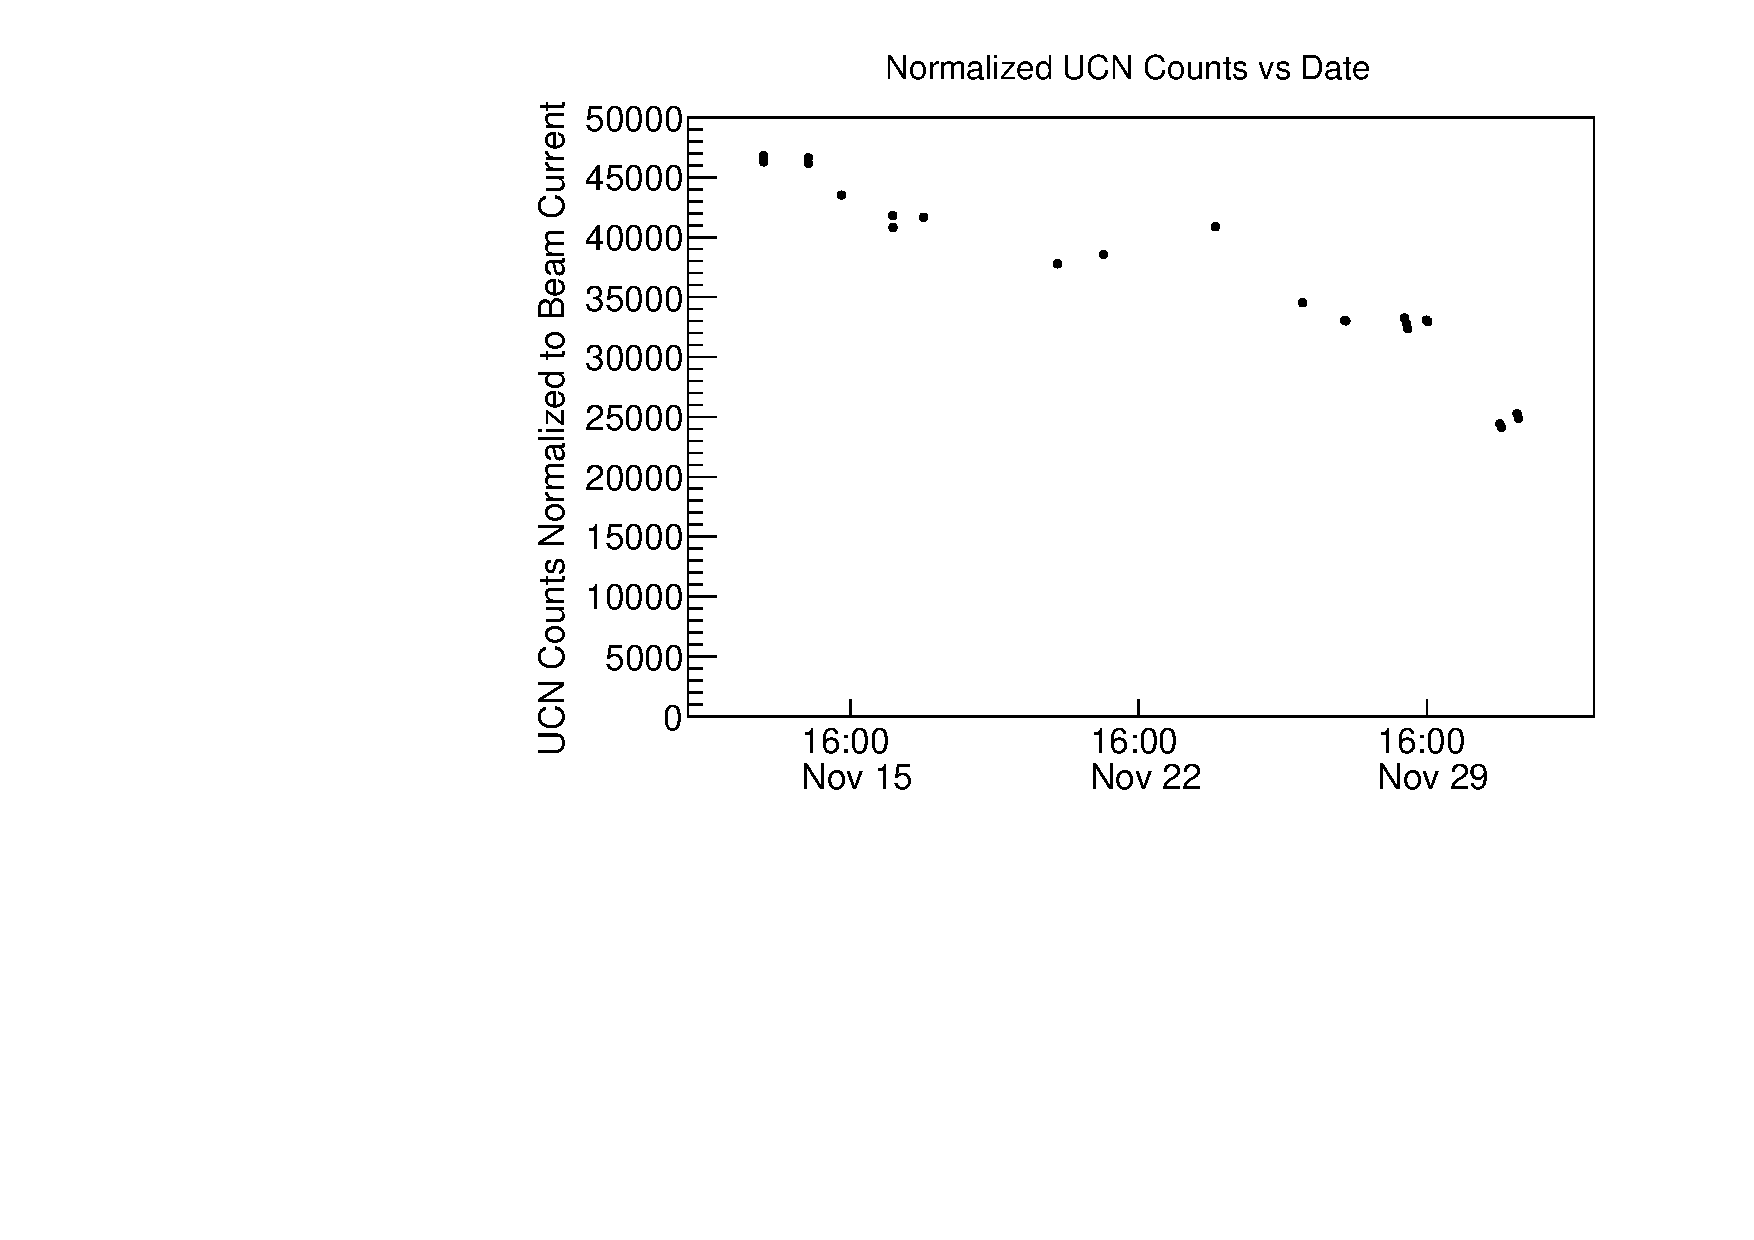
\includegraphics[width=0.9\textwidth]{UCNCounts_vs_time.pdf}
  \caption{The total UCN counts extracted from the source for 1~$\mu$A
    beam current and 60~s irradiation time at different days during
    the experimental run. }
  \label{fig:UCNCounts_time}
\end{figure}

\section{UCN Storage Lifetime~\label{storagelifetime}}

The total number of detected UCN strongly depends on the storage
lifetime of the source $\tau_1$~(see Eqn.~\ref{eqn:tau1}) which
indicates the performance of the UCN source. The storage lifetime of
UCN is determined by measuring the detected UCN at different valve
open delay times right after the irradiation stops.  The typical
chosen values are 0~s, 5~s, 10~s, 20~s, 30~s, 60~s, 80~s, 120~s and
170~s.
% For most of the experiments, the order in which the delay to the
% valve open time was applied was as following: 0~s, 170~s, 20~s,
% 120~s, 50~s, 80~s, 30~s and 5~s.
The exponential decay constant in the fit to the total UCN counts
without the background, for different valve open delay times, is the
total storage lifetime in the source.

Fig.~\ref{fig:storage_all} shows several UCN cycles for the standard
1~$\mu$A proton beam current and 60~s target irradiation time. The
difference in the maximum detected UCN rate is due to different valve
open delay times.
\begin{figure}[h!]
  \centering
  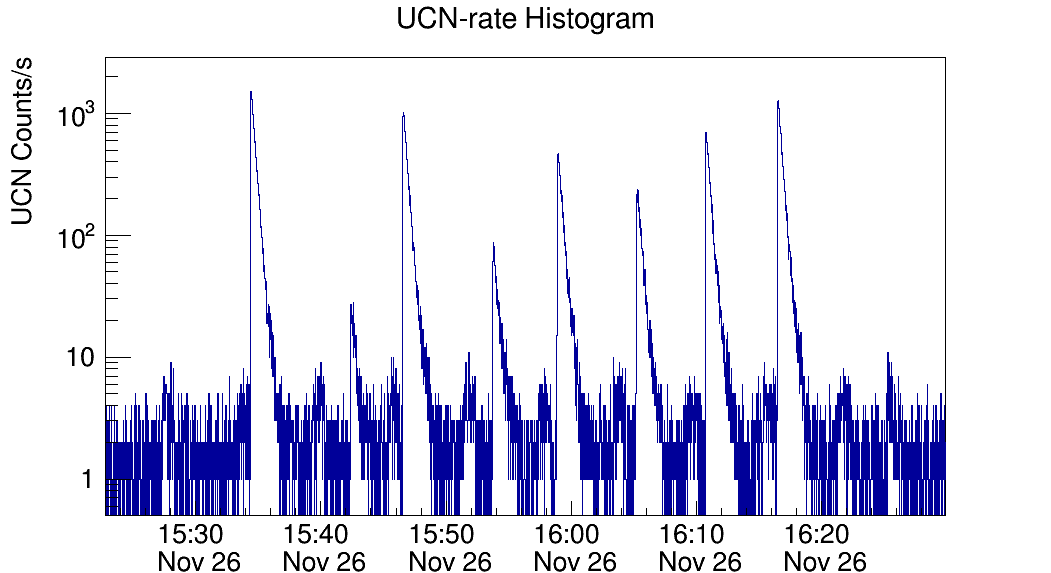
\includegraphics[width=0.9\textwidth]{storagetime_all.png}
  \caption{UCN cycles at different valve open delay times for 1~$\mu$A
    beam current and 60~s target irradiation time.}
  \label{fig:storage_all}
\end{figure}
Fig.~\ref{fig:storage_example} shows the total UCN counts~(background
subtracted) versus the valve open delay time for 1~$\mu$A proton beam
current and 60~s target irradiation time. The longer delay times give
rise to lower UCN counts due to the loss mechanisms. The one
exponential fit function
\begin{equation}
\text{UCN counts} = A e^{-t/\tau_1}~,
\end{equation}
determines the storage lifetime $\tau_1$. At 170~s valve open delay
time, the total UCN counts are not consistent with what the fit
function predicts due to low statistics. However, the result of the
fit is not driven by this inconsistency as it has a negligible effect
on the extrected storage lifetime.
%\begin{figure}[h!]
%  \centering
%  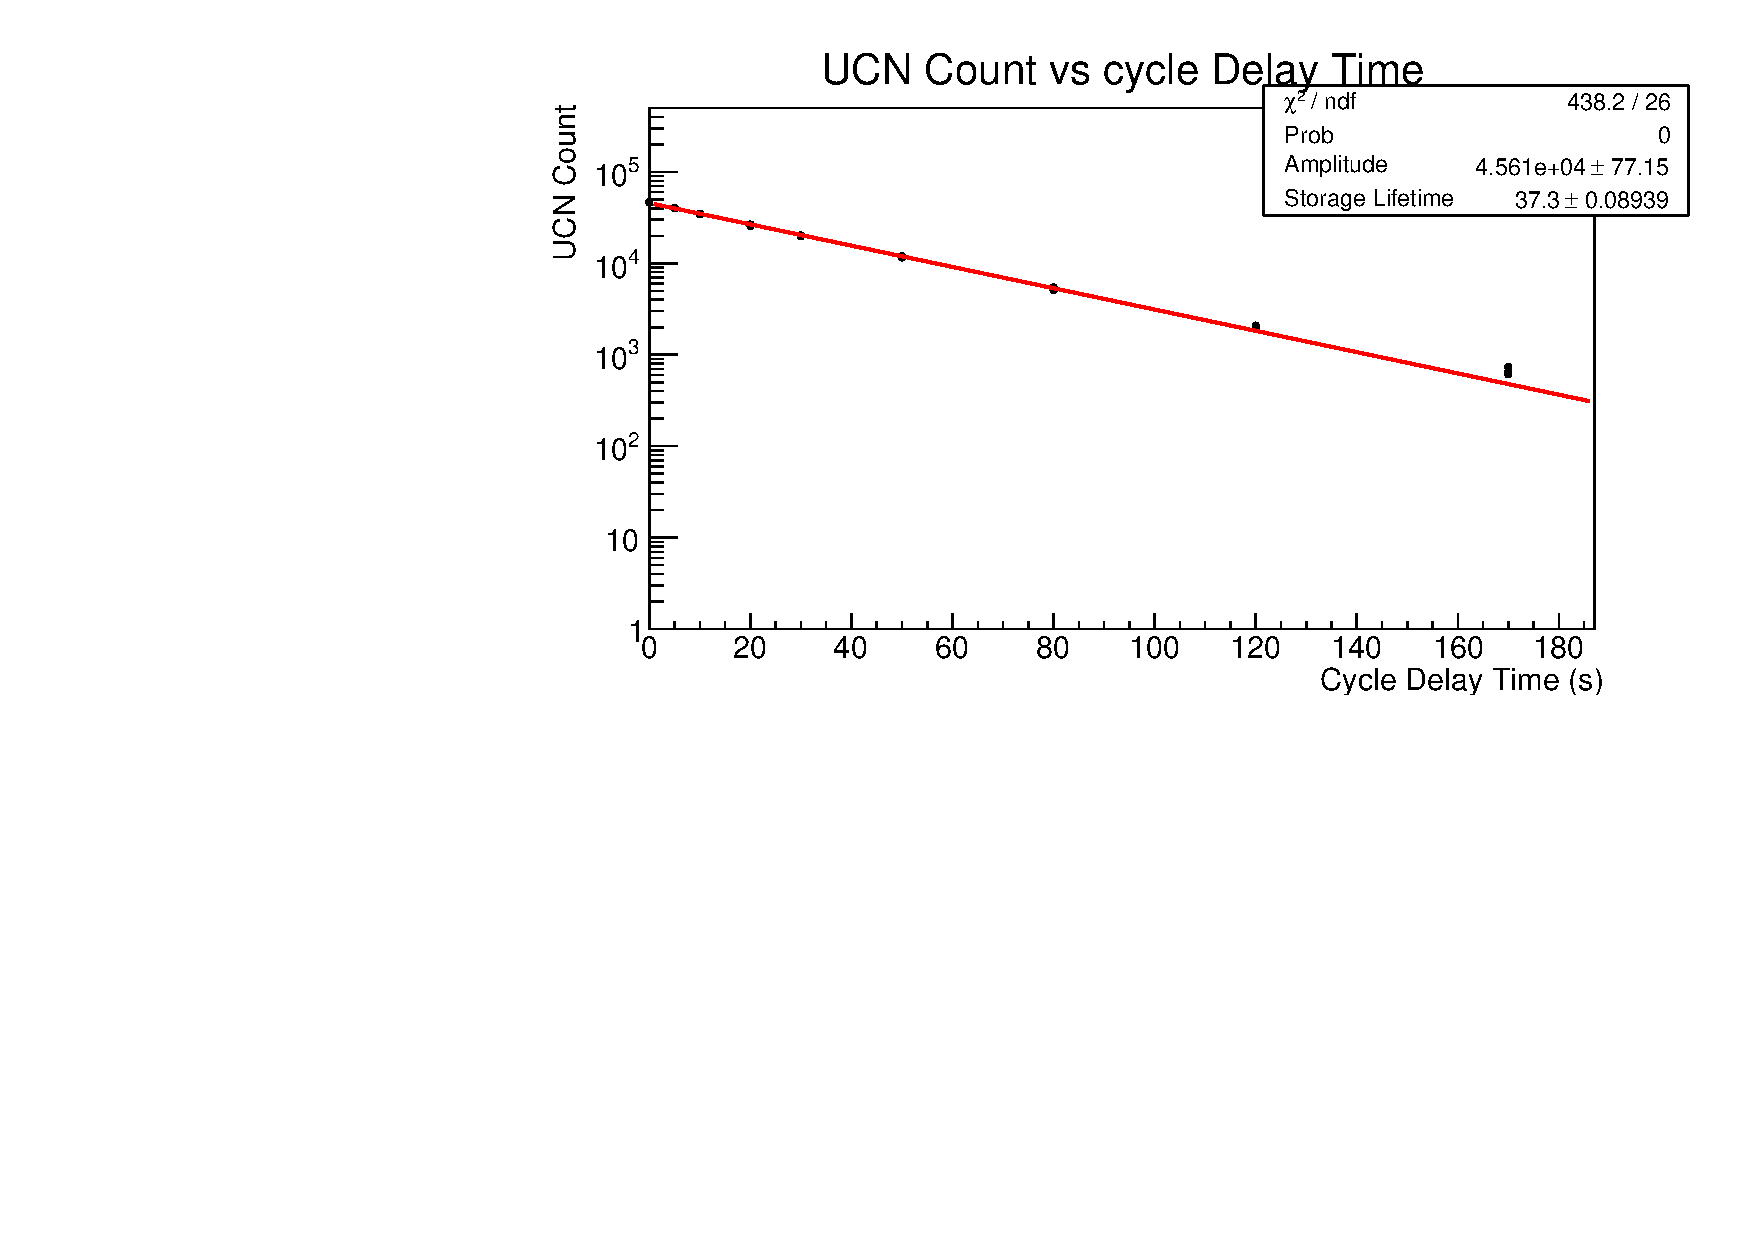
\includegraphics[width=0.9\textwidth]{17002_StorageLifetime.pdf}
%  \caption{The total UCN counts at different valve open delay times
%    for 1~$\mu$A beam current and 60~s irradiation time. The red line
%    is the one exponential fit. }
%  \label{fig:storage_example}
%\end{figure}

%\setlength\belowcaptionskip{-3ex}
\begin{figure}[h!]
  \centering
  \begin{subfigure}{.8\textwidth}
    \centering
    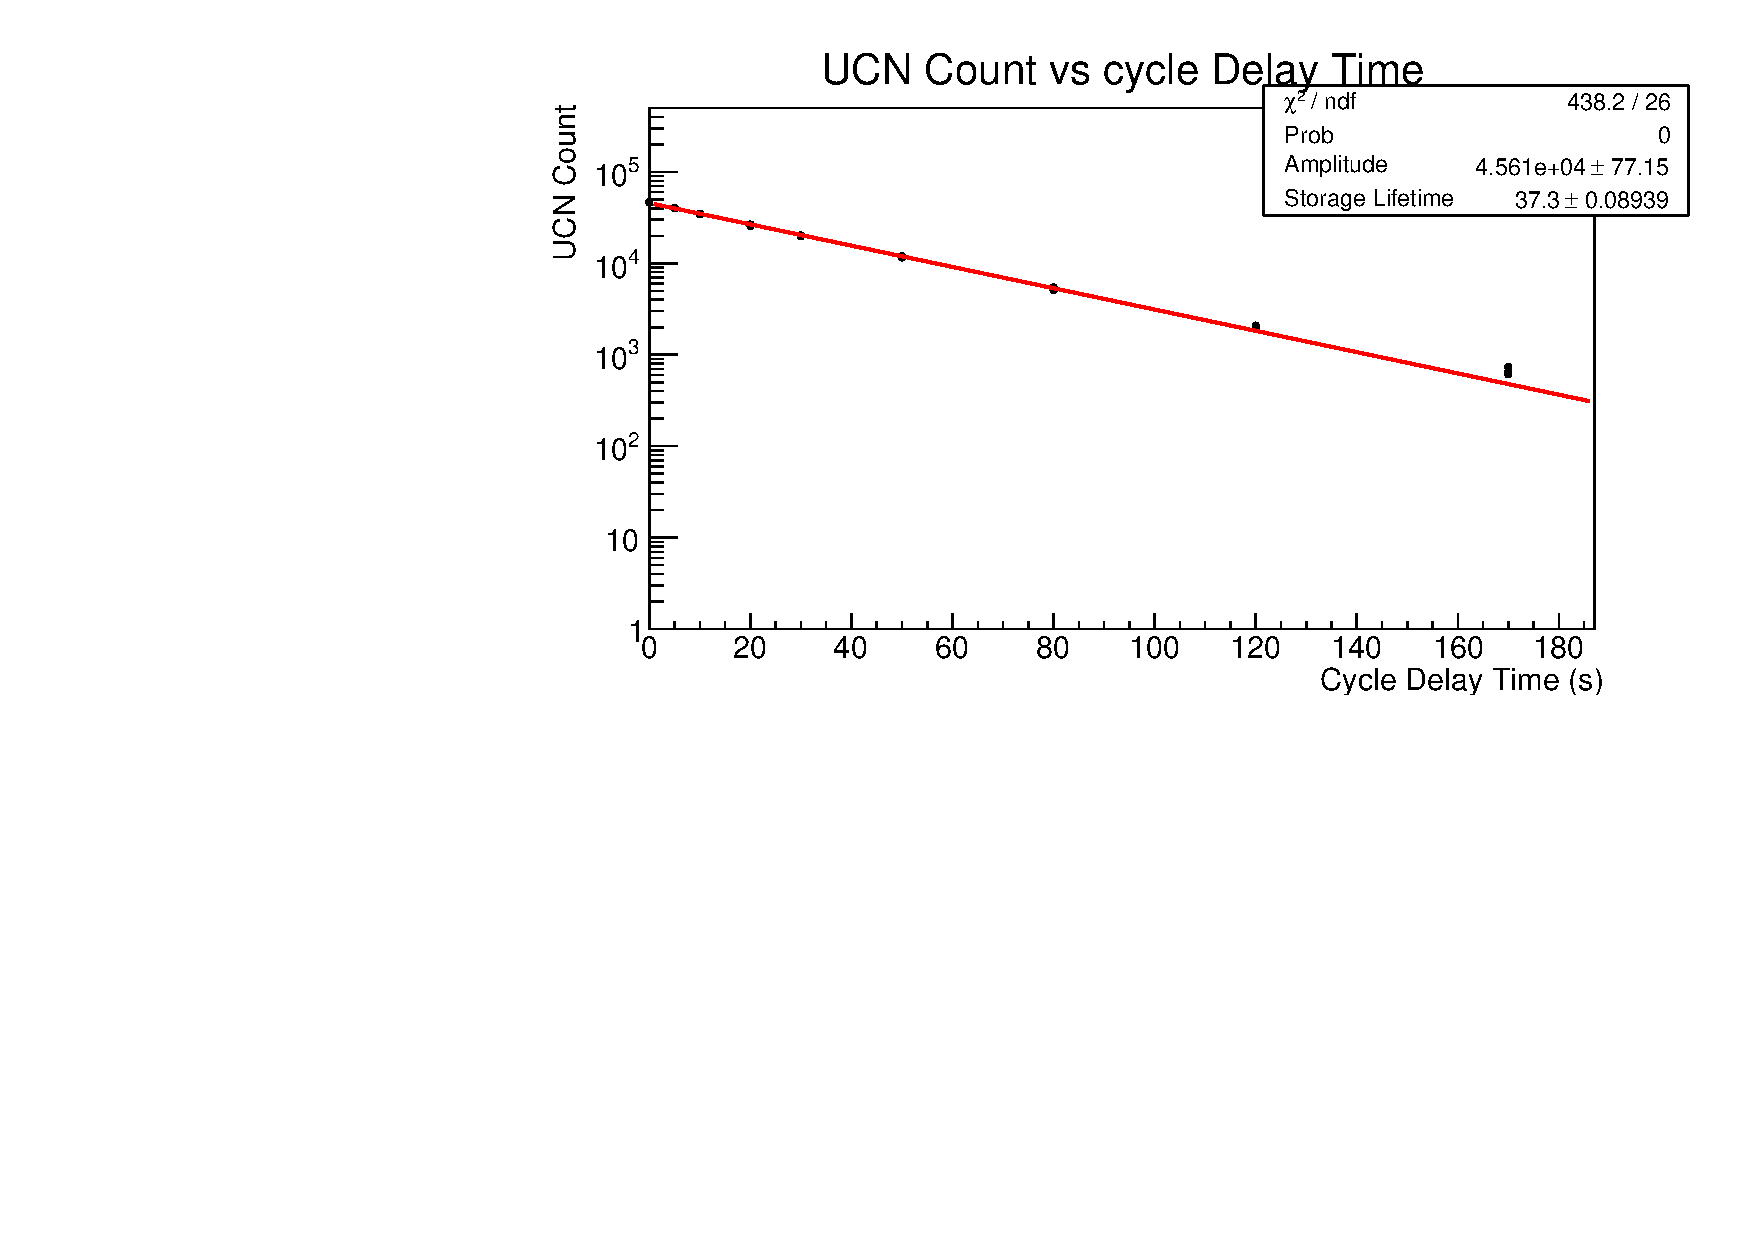
\includegraphics[width=1.0\textwidth]{17002_StorageLifetime.pdf}
    \caption{}
    \label{fig:storage_example1}
  \end{subfigure}%
  \\
  \begin{subfigure}{.8\textwidth}
    \centering
    \includegraphics[width=1.0\textwidth]{10muA_30s.pdf}
    \caption{}
    \label{fig:storage_example10}
  \end{subfigure}
  \caption{The total UCN counts at different valve open delay times for
    (a) 1~$\mu$A beam current and 60~s irradiation time and (b)
    10~$\mu$A beam current and 30~s target irradiation time. The red
    line is the one exponential fit. The initail UCN counts for the
    10~$\mu$A target irradiation is higher. However, the storage
    lifetime is lower compared to 1~$\mu$A beam current because of the
    heat load on the superfluid helium. In the case of 10~$\mu$A beam
    current, the maximum cycle delay time is 120~s compared to the 170~s
    delay time in the case of 1~$\mu$A beam current. This is due to
    excessive heat load on the cryostat and low statistics.}
  \label{fig:storage_example}
\end{figure}

%Below the result of the storage lifetime measurements are presented.

\subsection{Storage Lifetime Versus Beam Current and Irradiation Time}
The storage lifetime of UCN in the source is measured at different
proton beam currents and different target irradiation times for better
optimization of the source. The result of those measurements is shown
in Fig.~\ref{fig:storage_beam_irrad}. Here the vertical axis shows the
storage lifetime in the source in seconds, and the horizontal axis
shows the proton beam current in $\mu$A. Each marker represents a
target irradiation time. At lower beam currents, the duration of the
target irradiation does not make a significant difference in the
storage lifetime. At higher proton beam currents, the longer the
irradiation time takes, the lower the storage lifeimte will be.

In summary, irradiating the target at high proton beam currents and
longer irradiation times create a higher heat load on the UCN source,
which leads to higher upscattering rates, and as a result, lower UCN
storage lifetime in the source.

\begin{figure}[h!]
  \centering
  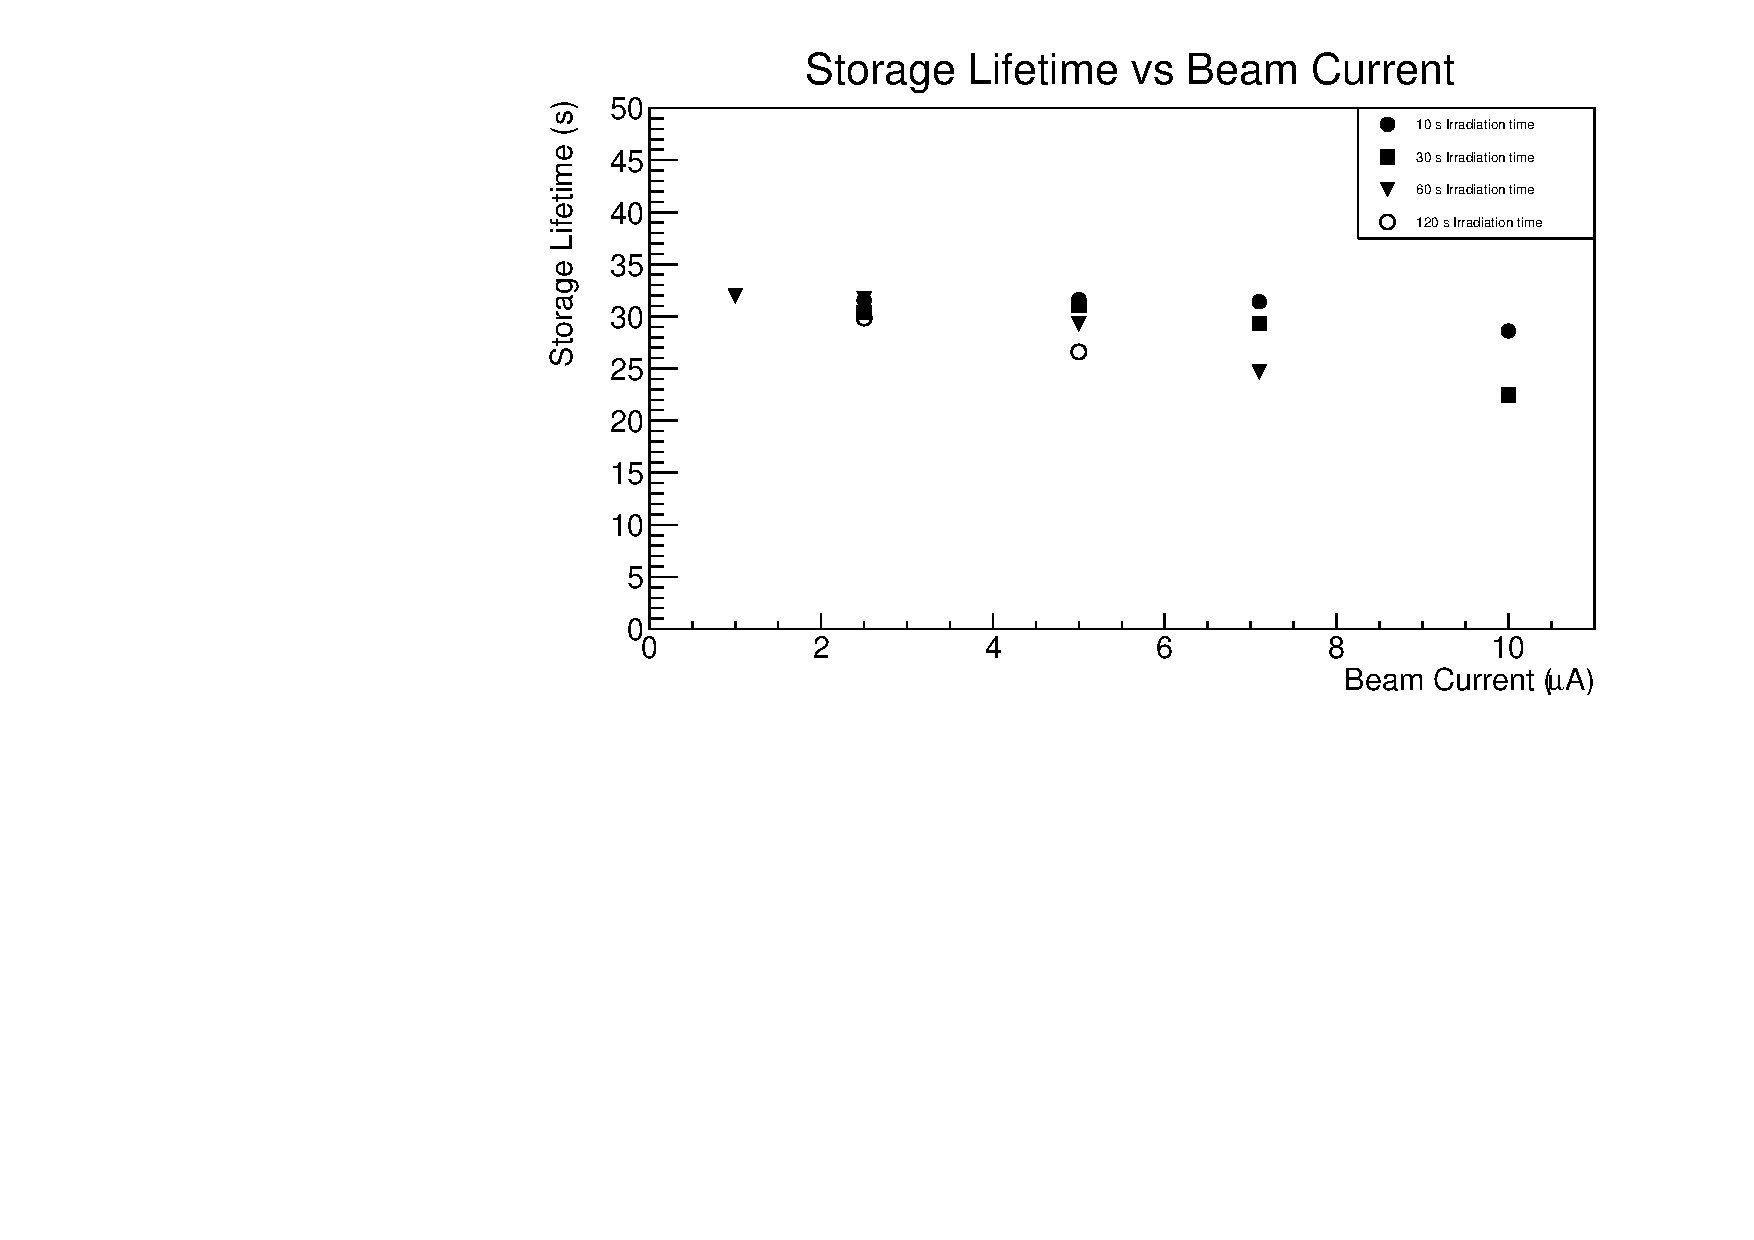
\includegraphics[width=0.9\textwidth]{StorageLifetime_17009_and_17009A.pdf}
  \caption{Storage lifetime in the source at different irradiation
    times and proton beam currents. Different markers refer to
    different target irradiation times. At longer irradiation times
    and higher beam currents, the storage lifetime decreases due to the
    increased heat load in the source, and an increase in the
    superfluid helium temperature. }
  \label{fig:storage_beam_irrad}
\end{figure}


\subsection{Storage Lifetime Versus Isopure Helium Temperature}
The storage lifetime of UCN was also measured at different
temperatures of the superfluid helium. In this experiment, the
temperature of superfluid was increased by using the heater tapes
wrapped around the UCN bottle. The heater powers were set to increase
the temperatures by a certain amount. Once the temperatures reached a
stable state, the target irradiation started.

The result of this measurement is shown in
Fig.~\ref{fig:storagelifetime_vs_temp}. The vertical axis is the
storage lifetime of UCN in seconds, and the horizontal axis is the
temperature of the superfluid helium. As mentioned earlier, the four
temperature sensors that measure the temperature of the superfluid
show some discrepancy. As a result, for a given value of the storage
lifetime, there are four different values for the temperature of the
superfluid. The vertical error bars are equal to $\sqrt{N}$, and the
horizontal error bars are set as
($T_{\mathrm{max}} - T_{\mathrm{min}}$)/2, as discussed earlier. The
data shows a downward trend. As the temperature of the superfluid
helium increases, the storage lifetime in the source decreases. This
is due to higher upscattering rate in the superfluid helium at
higher temperatures.


%TCN17014
\begin{figure}[h!]
  \centering
  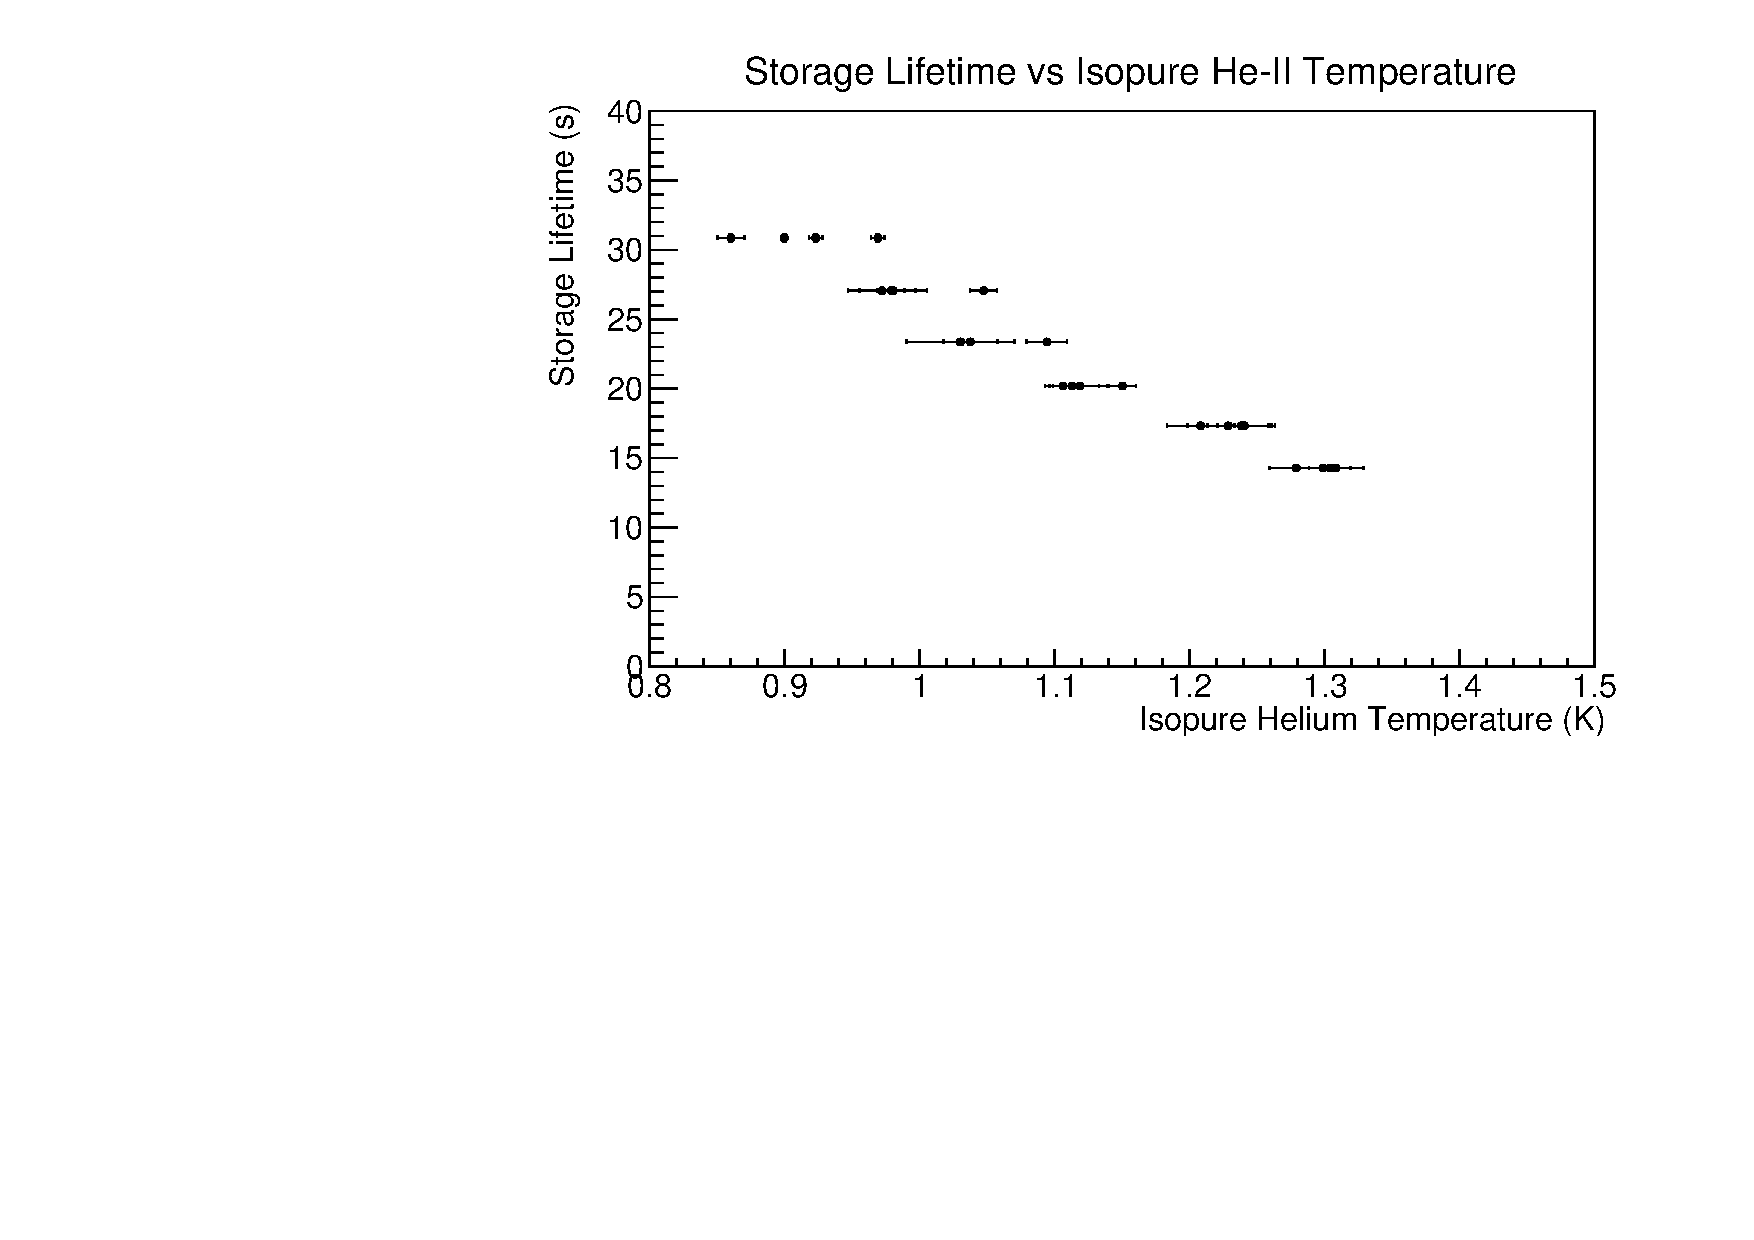
\includegraphics[width=0.9\textwidth]{StorageLifetime_vs_temp.pdf}
  \caption{Storage lifetime of UCN at different isopure helium
    temperatures. In this experiment, the temperature of the
    superfluid helium was set using heater tapes around the UCN
    bottle. The vertical axis shows the storage lifetime in seconds
    and the horizontal axis shows the superfluid helium temperature in
    Kelvin. As the temperature increases, the storage lifetime
    decreases. This is due to higher upscattering rate in the
    superfluid helium at higher temperatures.}
  \label{fig:storagelifetime_vs_temp}
\end{figure}



\subsection{Storage Lifetime Over Experimental Period\label{sec:storage_overall}}

The standard storage lifetime measurements were performed on a daily
basis over the course of the experimental run. This includes the
irradiation of the target at 1~$\mu$A proton beam current for
60~s. The result of those measurements are shown in
Fig.~\ref{fig:storagelifetime_overall}. Over a two week period, the
storage lifetime decreased from 37~s to 27~s. This is possibly due to
the contamination in the UCN source after opening the UCN valve.


\begin{figure}[h!]
  \centering
  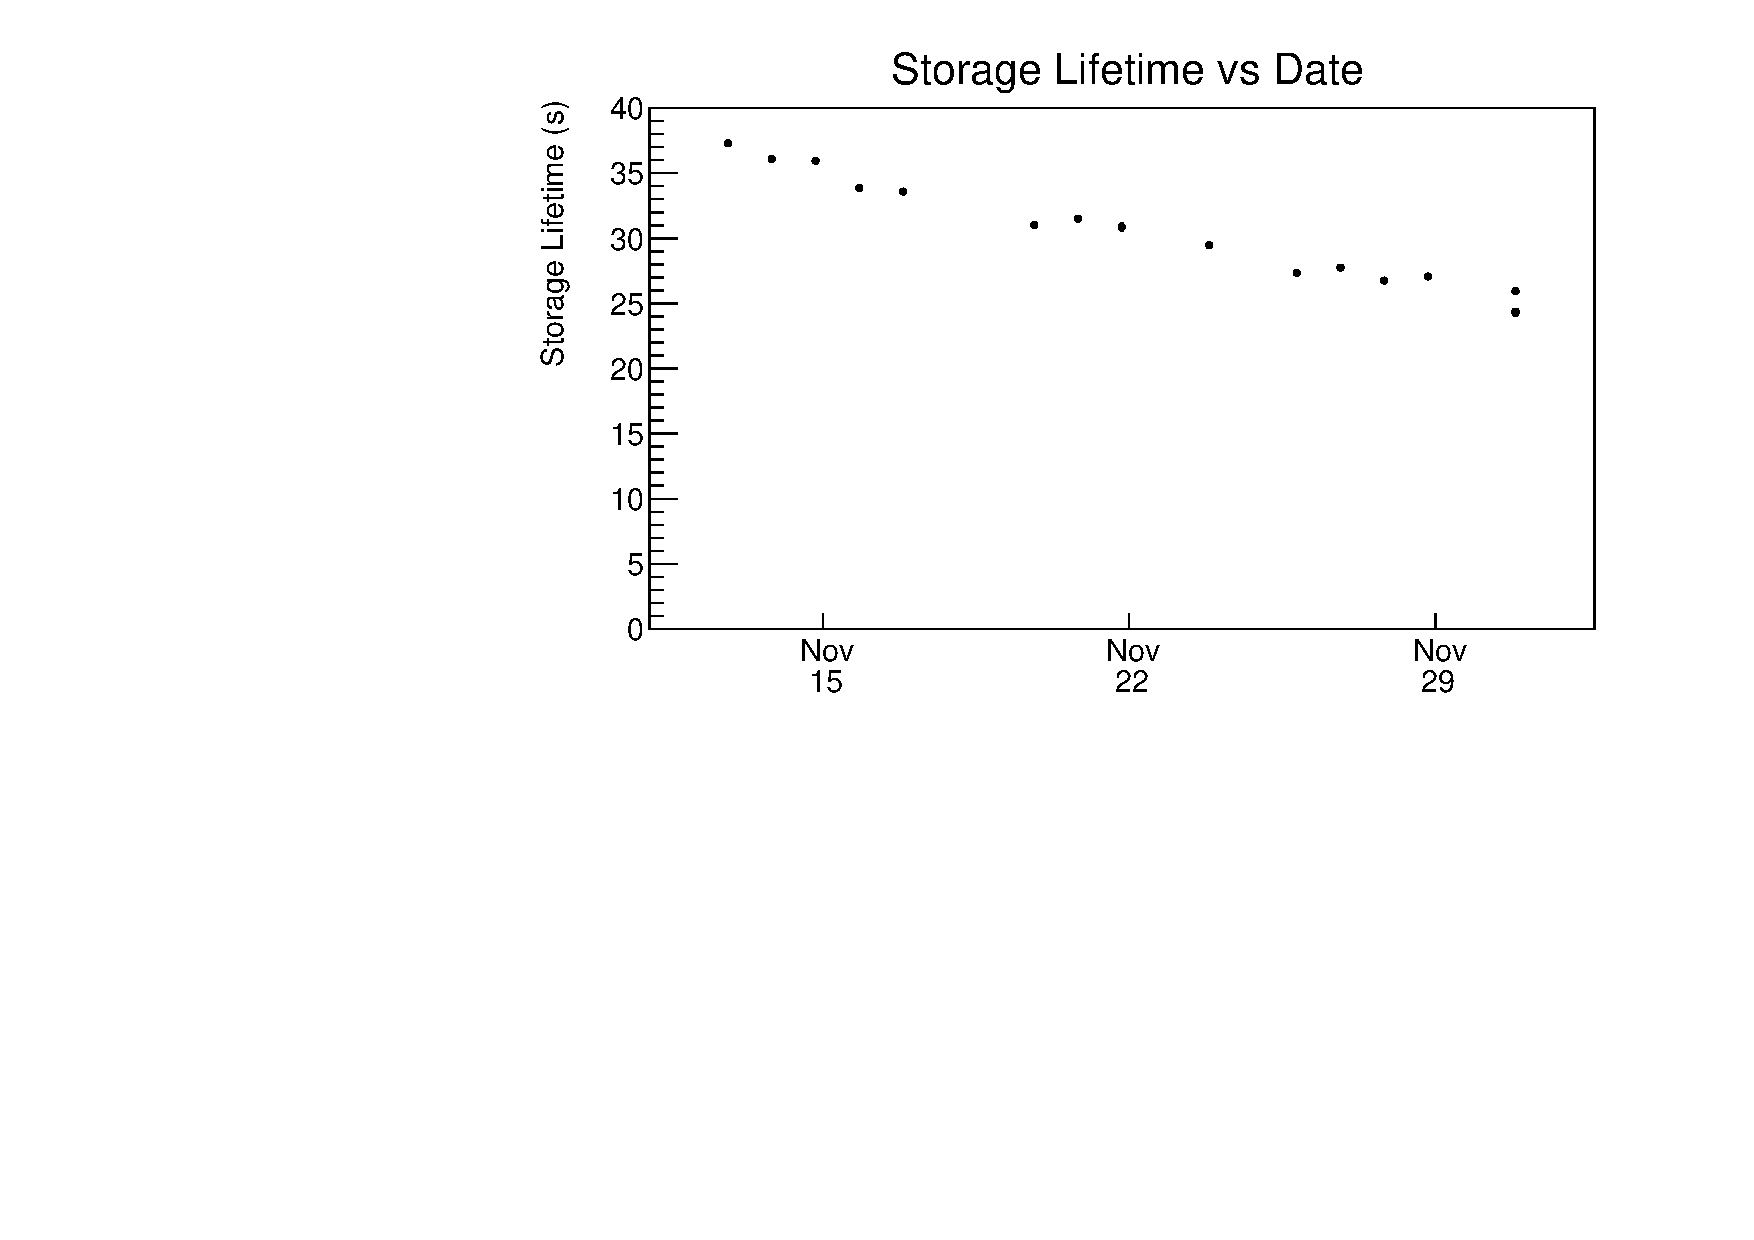
\includegraphics[width=0.9\textwidth]{storageLifetime_vs_time.pdf}
  \caption{Storage lifetime of the source over the experimental run. A
    2\% daily decrease in the storage lifetime is observed possibly
    due to the contamination in the source after opening the UCN
    valve.}
  \label{fig:storagelifetime_overall}
\end{figure}



\section{Main Results\label{sec:pentrack}}

For better understanding of the loss mechanisms of UCN, the
experiments were also simulated in
PENTrack~\cite{schreyer2017pentrack}. PENTrack is a particle tracking
simulation software which simulates the trajectories of UCN and their
decay products~(e.g., protons and electrons) and their spin precession
in complex geometries in Electric and Magnetic fields by solving the
relativistic equation of motion.

To simulate the UCN storage and transport, an exact model of the UCN
guides for PENTrack was build by the TUCAN team. Here the result of
those simulations and comparison to the measured data are presented.
%%%%%%%
\subsection{UCN Guide Diffusivity\label{sec:diffusivity}}
As discussed in Chapter~\ref{chap:intro}, UCN interact with all four
fundamental forces. To describe the interaction of UCN with matter, a
complex optical potential is used to describe matters:
\begin{equation}
  \label{eqn:fermipotential}
  U = V - iW
\end{equation}
where the real part, $V$, depends on the number densities and bound
coherent scattering lengthes of each nucleus species. The imaginary
part, $W$, depends on the loss cross-section for a given velocity.
Upon the incidence of a UCN on a surface, it can be scatterd either
specularly or diffusely. The specular reflection by definition is the
reflection of light from a smooth surface at a defined angle. The
diffuse reflection is the reflection by rough surfaces that tend to
reflect light in all directions.

PENTrack simulations were performed to extract the diffusivity of the
UCN guides~(see Fig.~\ref{fig:Source_all}). PENTrack uses two models
to calculate the scattering distribution of the UCN impinging on the
material surface: Lambert model or the
Microroughness~\cite{Steyerl1972}. Experimental geometries imported in
PENTrack are the StL files made through CAD models. For these
simulations, the exact model of the vertical UCN source was used
including the burst disk, the actual shape of the UCN valve in the
open and close state, pinhole, foil and the detector~(see
Section~\ref{sec:vertical_source} for more details).

The abosorption in the foil is set according to the measurements
in~\cite{atchison2009transmission}. The main detector is modeled with
its two scintillator layers~\cite{jamieson2017characterization} and
their corresponding Fermi potentials and absorption cross-section, as
stated in~\cite{Ban2016}. In the simulations, it is assumed that the
spectrum of produced UCN is proportional to $\sqrt{E}$ and that the
upscattering rate in the superfluid helium follows
$\tau_\mathrm{He} = B T^7$ , with $B$ between 0.008~$s^{-1}$ and
0.016~$s^{-1}$ as measured by~\cite{Leung2016}. The wall loss
parameters were tuned to give a storge lifetime in the source $\tau_1$
between~($29.81 \pm 0.18$)~s and ($31.07 \pm 0.19$)~s matching the
storage lifetime during the middle of the experimental run, and
resulting in the material parameters shown in
Table~\ref{tab:materials}.


%$\tau_1 = 34.9 \pm .8$~s with an upscattering lifetime in the
%superfluid of
%$\tau_{\mathrm{He}}^{-1} = (390~\mathrm{s})^{-1} =
%0.008~\mathrm{s}^{-1}\cdot 0.85^{7}$, resulting in material parameters
%shown in Table~\ref{tab:materials}.


\begin{table}
  \centering
\begin{tabular}{|c|c|c|}
  \hline
Material & Fermi pot. (neV) & Diffusivity \\
\hline
  He-II  & $18.8 - 0.5\hbar B T^7 i$ & 0.16 \\
  He vapour & $-0.5 \hbar \tau^{-1}_\mathrm{vapour} i$ & 0 \\
  Prod. volume (NiP) & $213 - 0.120 i$ & 0.05 \\
  Guides (stainl. steel) & $183 - 0.140 i$ & 0.03 \\
  % Pinhole (copper) & $171 - 0.0726 i$ & 0.20 \\
  Foil (aluminium) & $54.1 - 0.00281 i$ & 0.20 \\
  GS30 scintillator & $83.1 - 0.000123 i$ & 0.16 \\
  GS20 scintillator & $103 - 1.24 i$ & 0.16 \\
  \hline
\end{tabular}
\caption{Material parameters used in PENTrack
  simulation.~\cite{atchison2009transmission,Ban2016,sears1992neutron}}
\label{tab:materials}
\end{table}

%%%%%%%%%%%%%% moved the helium gas stuff from here %%%%%%%%%%%%%%%%%%%%%%%%%

To better match the simulated UCN transport with reality, both the
simulation and the measured UCN rate in the detector after opening the
valve at $t=0$ are fitted with the function

\begin{equation}
R(t) = R_0 \left[ 1 - \exp \left( -\frac{t - \Delta t}{\tau_\mathrm{rise}} \right) \right] \exp \left( -\frac{t - \Delta t}{\tau_2} \right) + R_B
\end{equation}
In this equation, $\Delta t$ is the delay time between opening the
valve and detecting the first UCN and it is 2 to 3~s. The parameter
$R_B$ is the background UCN rate in the experimental data and is zero
in the simulations. The fit funciton, the rise time
$\tau_{\mathrm{rise}}$, and the fall time~$\tau_2$ are shown in
Fig.~\ref{fig:risefalltime} for a given UCN cycle.

In the simulations, the Lambert model is used to tune the probablity
of UCN being diffusely reflected on the guide walls to match the rise
time and fall time of the UCN rate in the storage lifetime
measurements~(see Fig.~\ref{fig:falltime} and
Fig.~\ref{fig:risetime}).  The delay time $\Delta t$ matches in all
scenarios.  In the graphs, the data is shown by the boxes and the
simulation results for different UCN guide diffusivity are shown by
different markers. The boxes indicate the second and third quartile of
the experimental data. Quartiles divide the data set to four
sections. The median of the data set is the second quartile. The value
between the minimum value of a data set and the median is the first
quartile. The value between the median and the maximum value of a data
set is the third quartile.

Diffuse reflection probabilities of 1\% and 10\% clearly result in too
short and too long time constants. The experimental fall time can be
matched with diffuse reflection probabilities of 3\% and 5\%. The rise
time is best matched with 3\%. This value is similar to values
reported for a range of UCN
guides~\cite{DAUM201471,Wlokka2017,Atchison2010}.


\begin{figure}[h!]
  \centering
  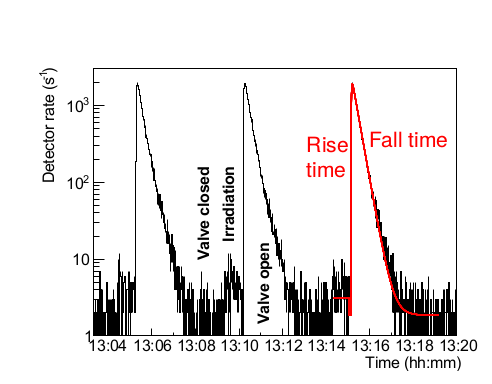
\includegraphics[width=0.8\textwidth]{risefalltime.png}
  \caption{UCN rate with two exponential fit shown in red. The rise
    time and fall time are labeled.}
  \label{fig:risefalltime}
\end{figure}

	
\begin{figure}[h!]
  \centering 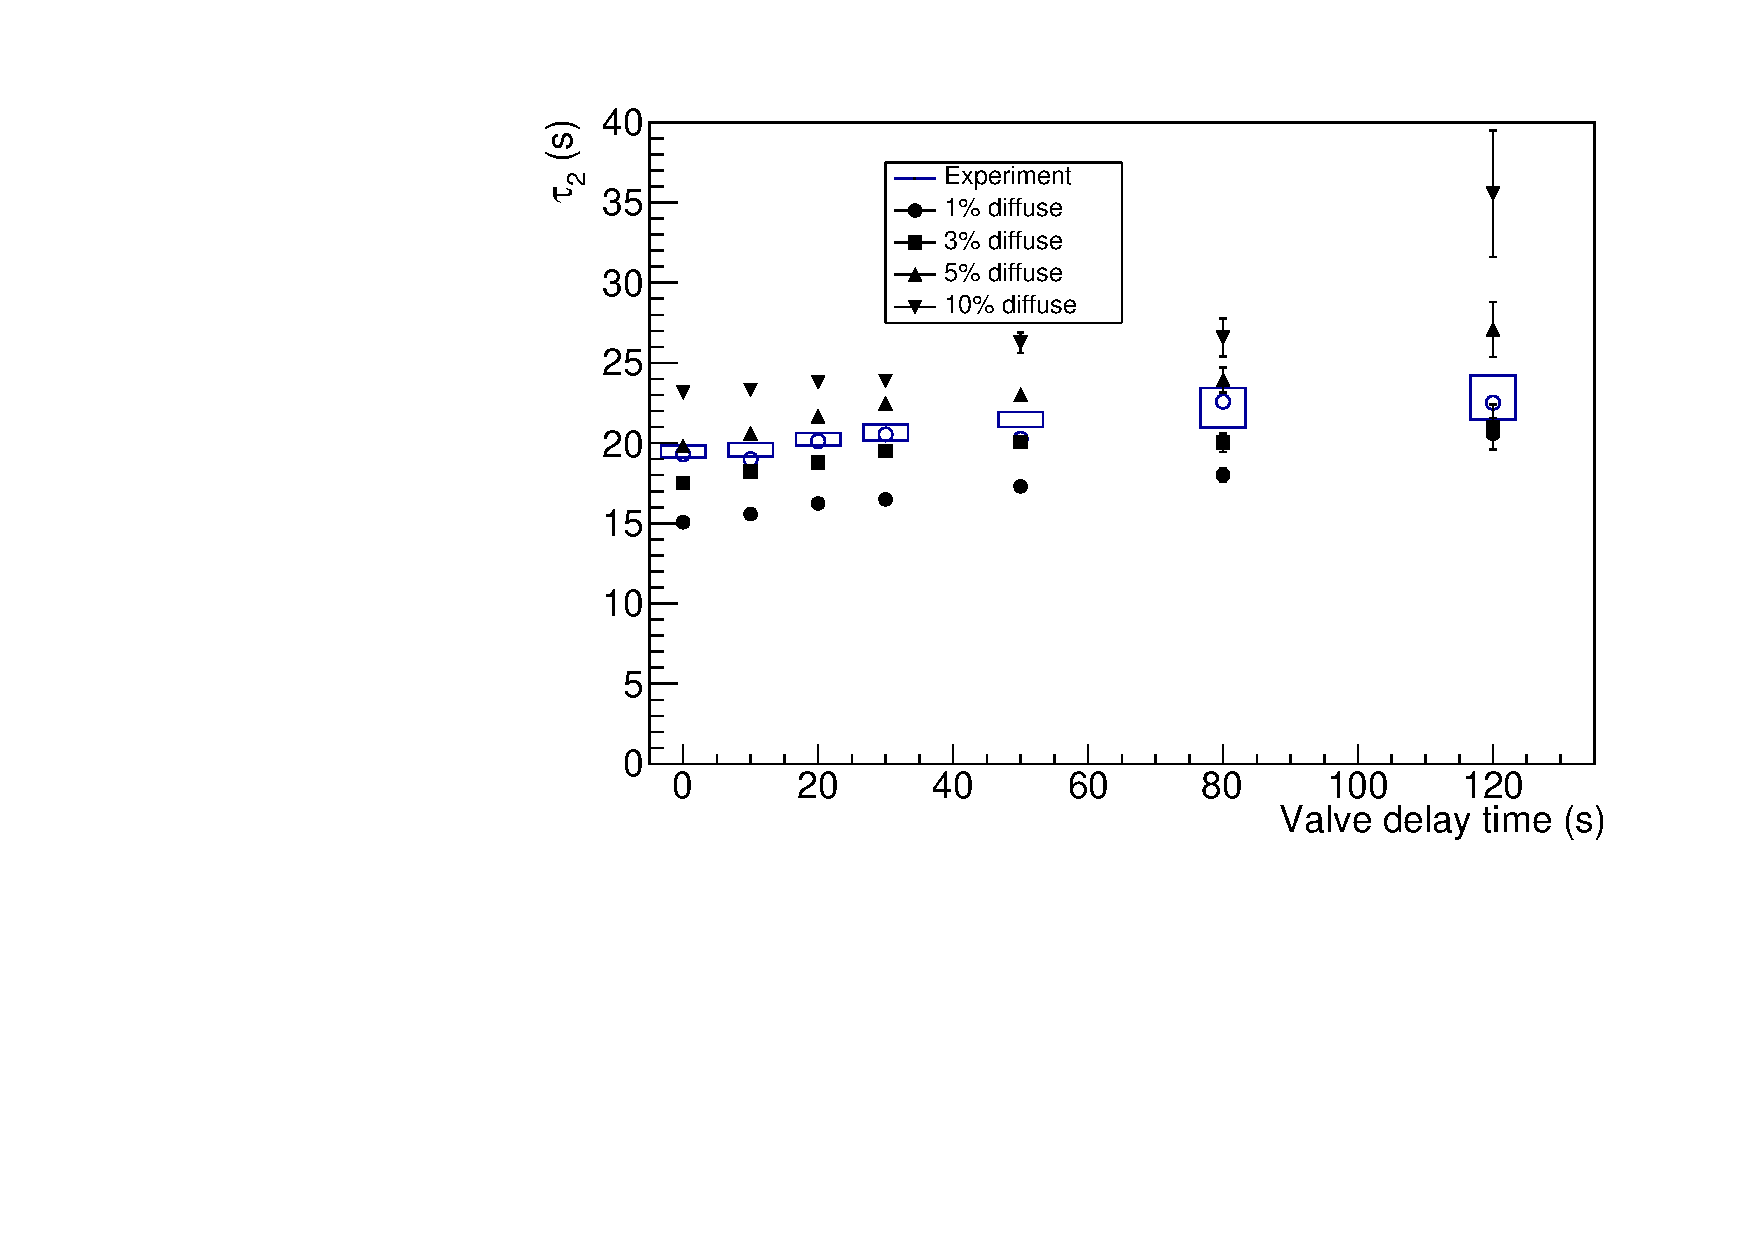
\includegraphics[width=0.9\textwidth]{falltime.pdf}
  \caption{Comparison of fall time $\tau_2$ in the experimental data
    and the simulations with different diffuse-reflection
    probabilities. The boxes indicate the second and third quartile of
    the experimental data~(see text for the definition of quartiles).
    The empty circle indicates its average.}
\label{fig:falltime}
\end{figure}

\begin{figure}[h!]
\centering
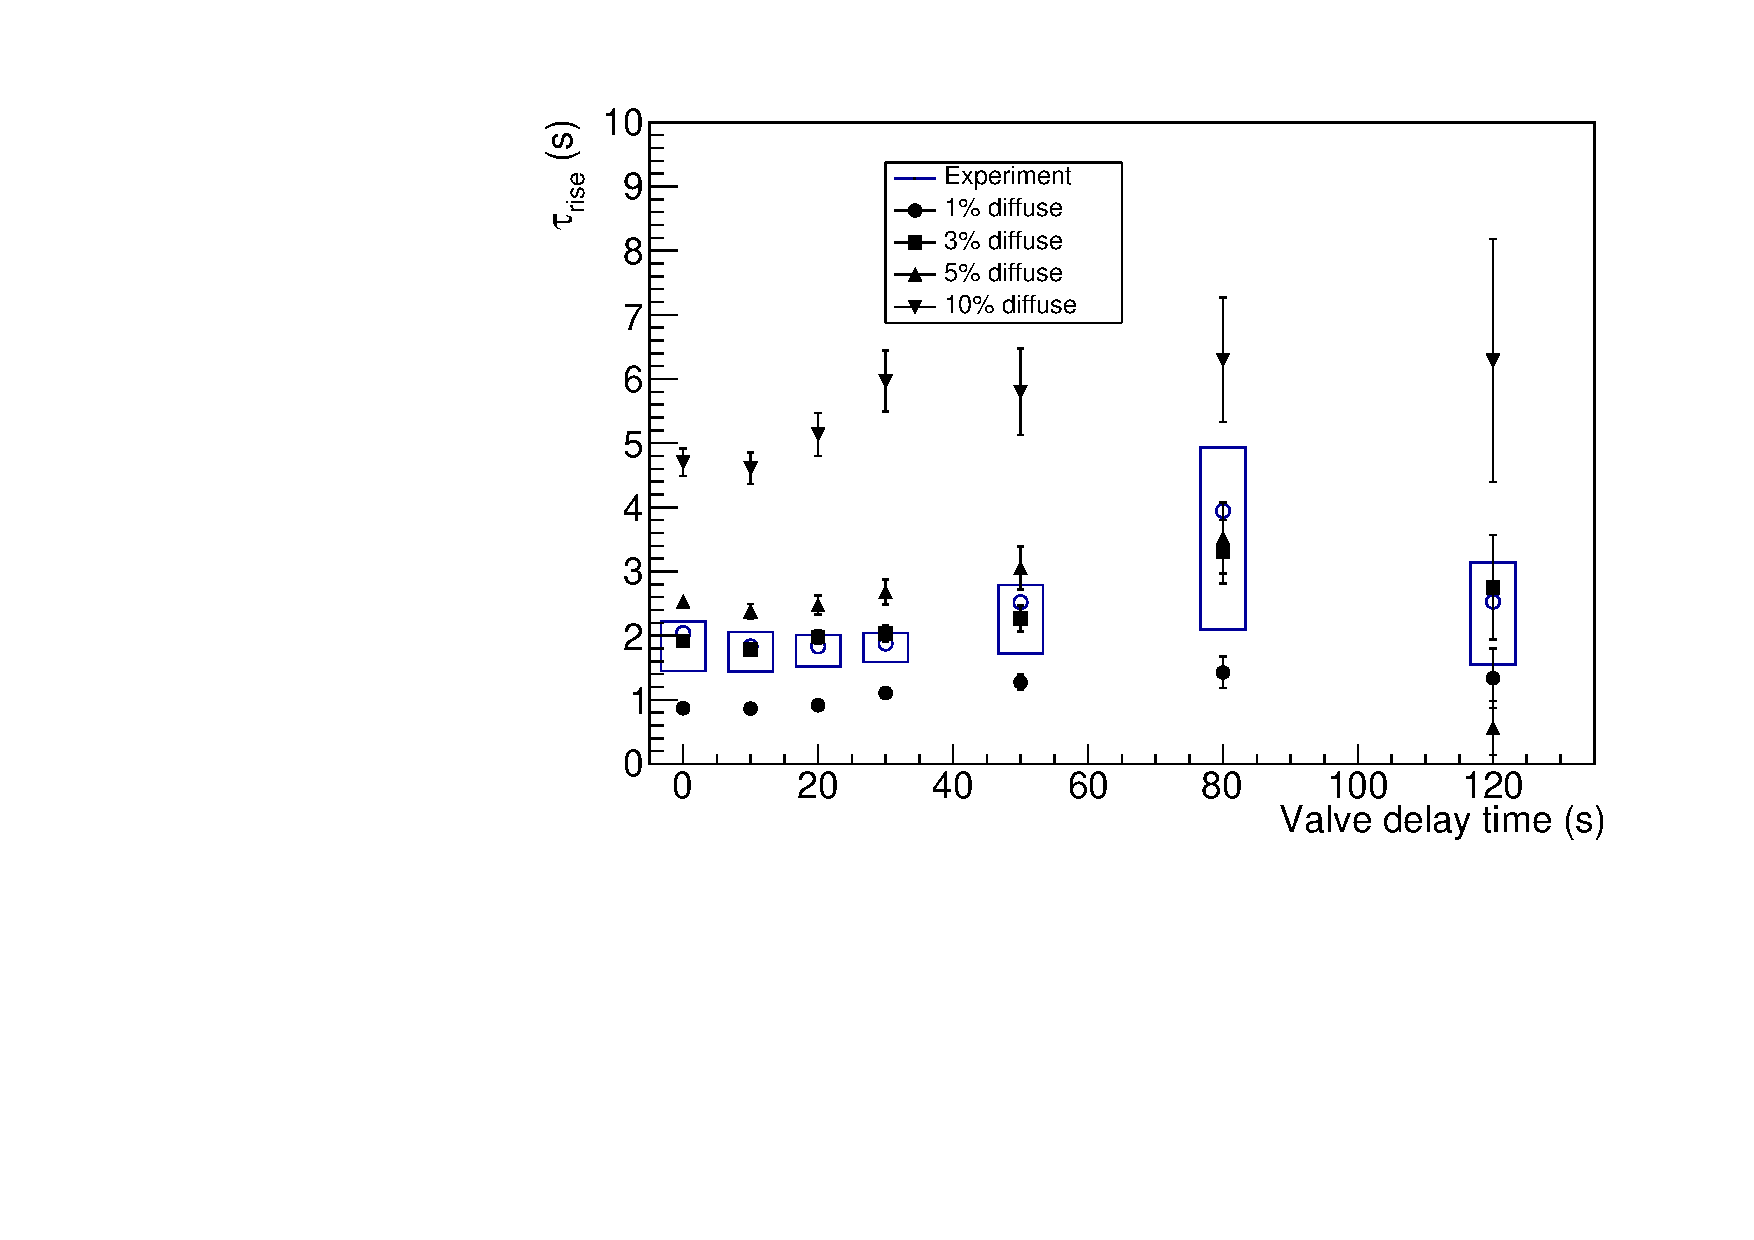
\includegraphics[width=0.9\textwidth]{risetime.pdf}
\caption{Comparison of rise time $\tau_{\mathrm{rise}}$ in
  experimental data and simulations with different diffuse-reflection
  probabilities. The boxes indicate the second and third quartile of
  the experimental data~(see text for the definition of
  quartiles). The empty circles indicate the average.}
\label{fig:risetime}
\end{figure}



%\subsection{UCN Upscattering Coefficient}
%The simulations are also used to determine the parameter
%$f_{\mathrm{He}}$ or the fraction of time that UCN spends in the
%superfluid helium in the detectable range of 120~neV to 200~neV.
%%%%How???
%For the steady-state measurements, this fraction turned out to be
%almost constant over a range of upscattering lifetime in the
%superfluid helium giving

%\begin{equation}
%f_\mathrm{He,3} = 0.464 \pm 0.001_\mathrm{stat.} \pm 0.003_\mathrm{syst.},
%\end{equation}
%where the systematic uncertainty is the variation in simulations with
%$\tau_{\mathrm{He}}$ from 3.05~s to 390~s. 
%The Eqn.~\ref{eqn:tau2} could be rewritten as
%\begin{equation}
%  \label{eqn:tau2rewritten}
%\tau_d^{-1} + \tau_\mathrm{wall,2}^{-1} = \tau_2^{-1}(T_0) - f_\mathrm{He,2} B \left( T_%0 \right)^a
%\end{equation}
%where the value for $\tau_2$ is
%\begin{equation}
%\tau_2^{-1}(T_0) = (19.3 \pm 0.8_\mathrm{stat.})\,~\si{\second}
%\end{equation}
%comes from fall time in the storage lifetime measurements at the
%temperature $T_0$ which is
%\begin{equation}
%T_0 = 0.92 \pm 0.005_\mathrm{stat.} \pm 0.05_\mathrm{syst.}.
%\end{equation}
%Replacing Eqn.~\ref{eqn:tau2rewritten} in Eqn.~\ref{eq:b}, $B$ can be written as
%\begin{equation}
%B = \frac{b \tau_2^{-1}(T_0)}{f_\mathrm{He,3} + f_\mathrm{He,2} b \left( \frac{T_0}{\SI{%1}{\kelvin}} \right)^a}.
%\end{equation}
%Here all the parameters are known except for $ f_\mathrm{He,2}$ which
%does not significantly affect the result, and hence, it is assumed to
%lie between 0 and 1. As a result
%\begin{equation}
%B = (10.4 \pm 0.4_\mathrm{stat.} \pm 4.1_\mathrm{syst.}) \cdot 10^{-3} \, \si{\per\second}.
%\end{equation}
%which is consistent with the result in~\cite{Leung2016}.


\subsection{UCN Yield and Storage Lifetime Simulations}
To estimate the UCN production, a model of accurate target, moderator
and UCN converter geometries were build for MCNP6.1, taking into
account material impurities determined from assays and fill levels of
liquid moderator vessels~(see Fig.~\ref{fig:mcnpmodel}). The full
source is then simulated: the proton beam hitting the target,
secondary neutrons, protons, photons, and electrons, and neutron
moderation in graphite and heavy water. In contrast to liquid heavy
water, there is no detailed data on thermal neutron scattering in
solid heavy water available. Instead, we relied on a free-gas model
with an effective temperature of 80~K, as this seems to be the minimum
effective neutron temperature achieved with solid heavy water
moderatores~\cite{rush1966}. From the simulated cold neutron flux in the UCN
production volume and UCN production cross sections
from~\cite{Schmidt2015,Korobkina2002}, a production rate of
($20600\pm 200$)~s$^{-1}$ in an energy range up to 233.5~neV was
determined.

\begin{figure}[h!]
  \centering
  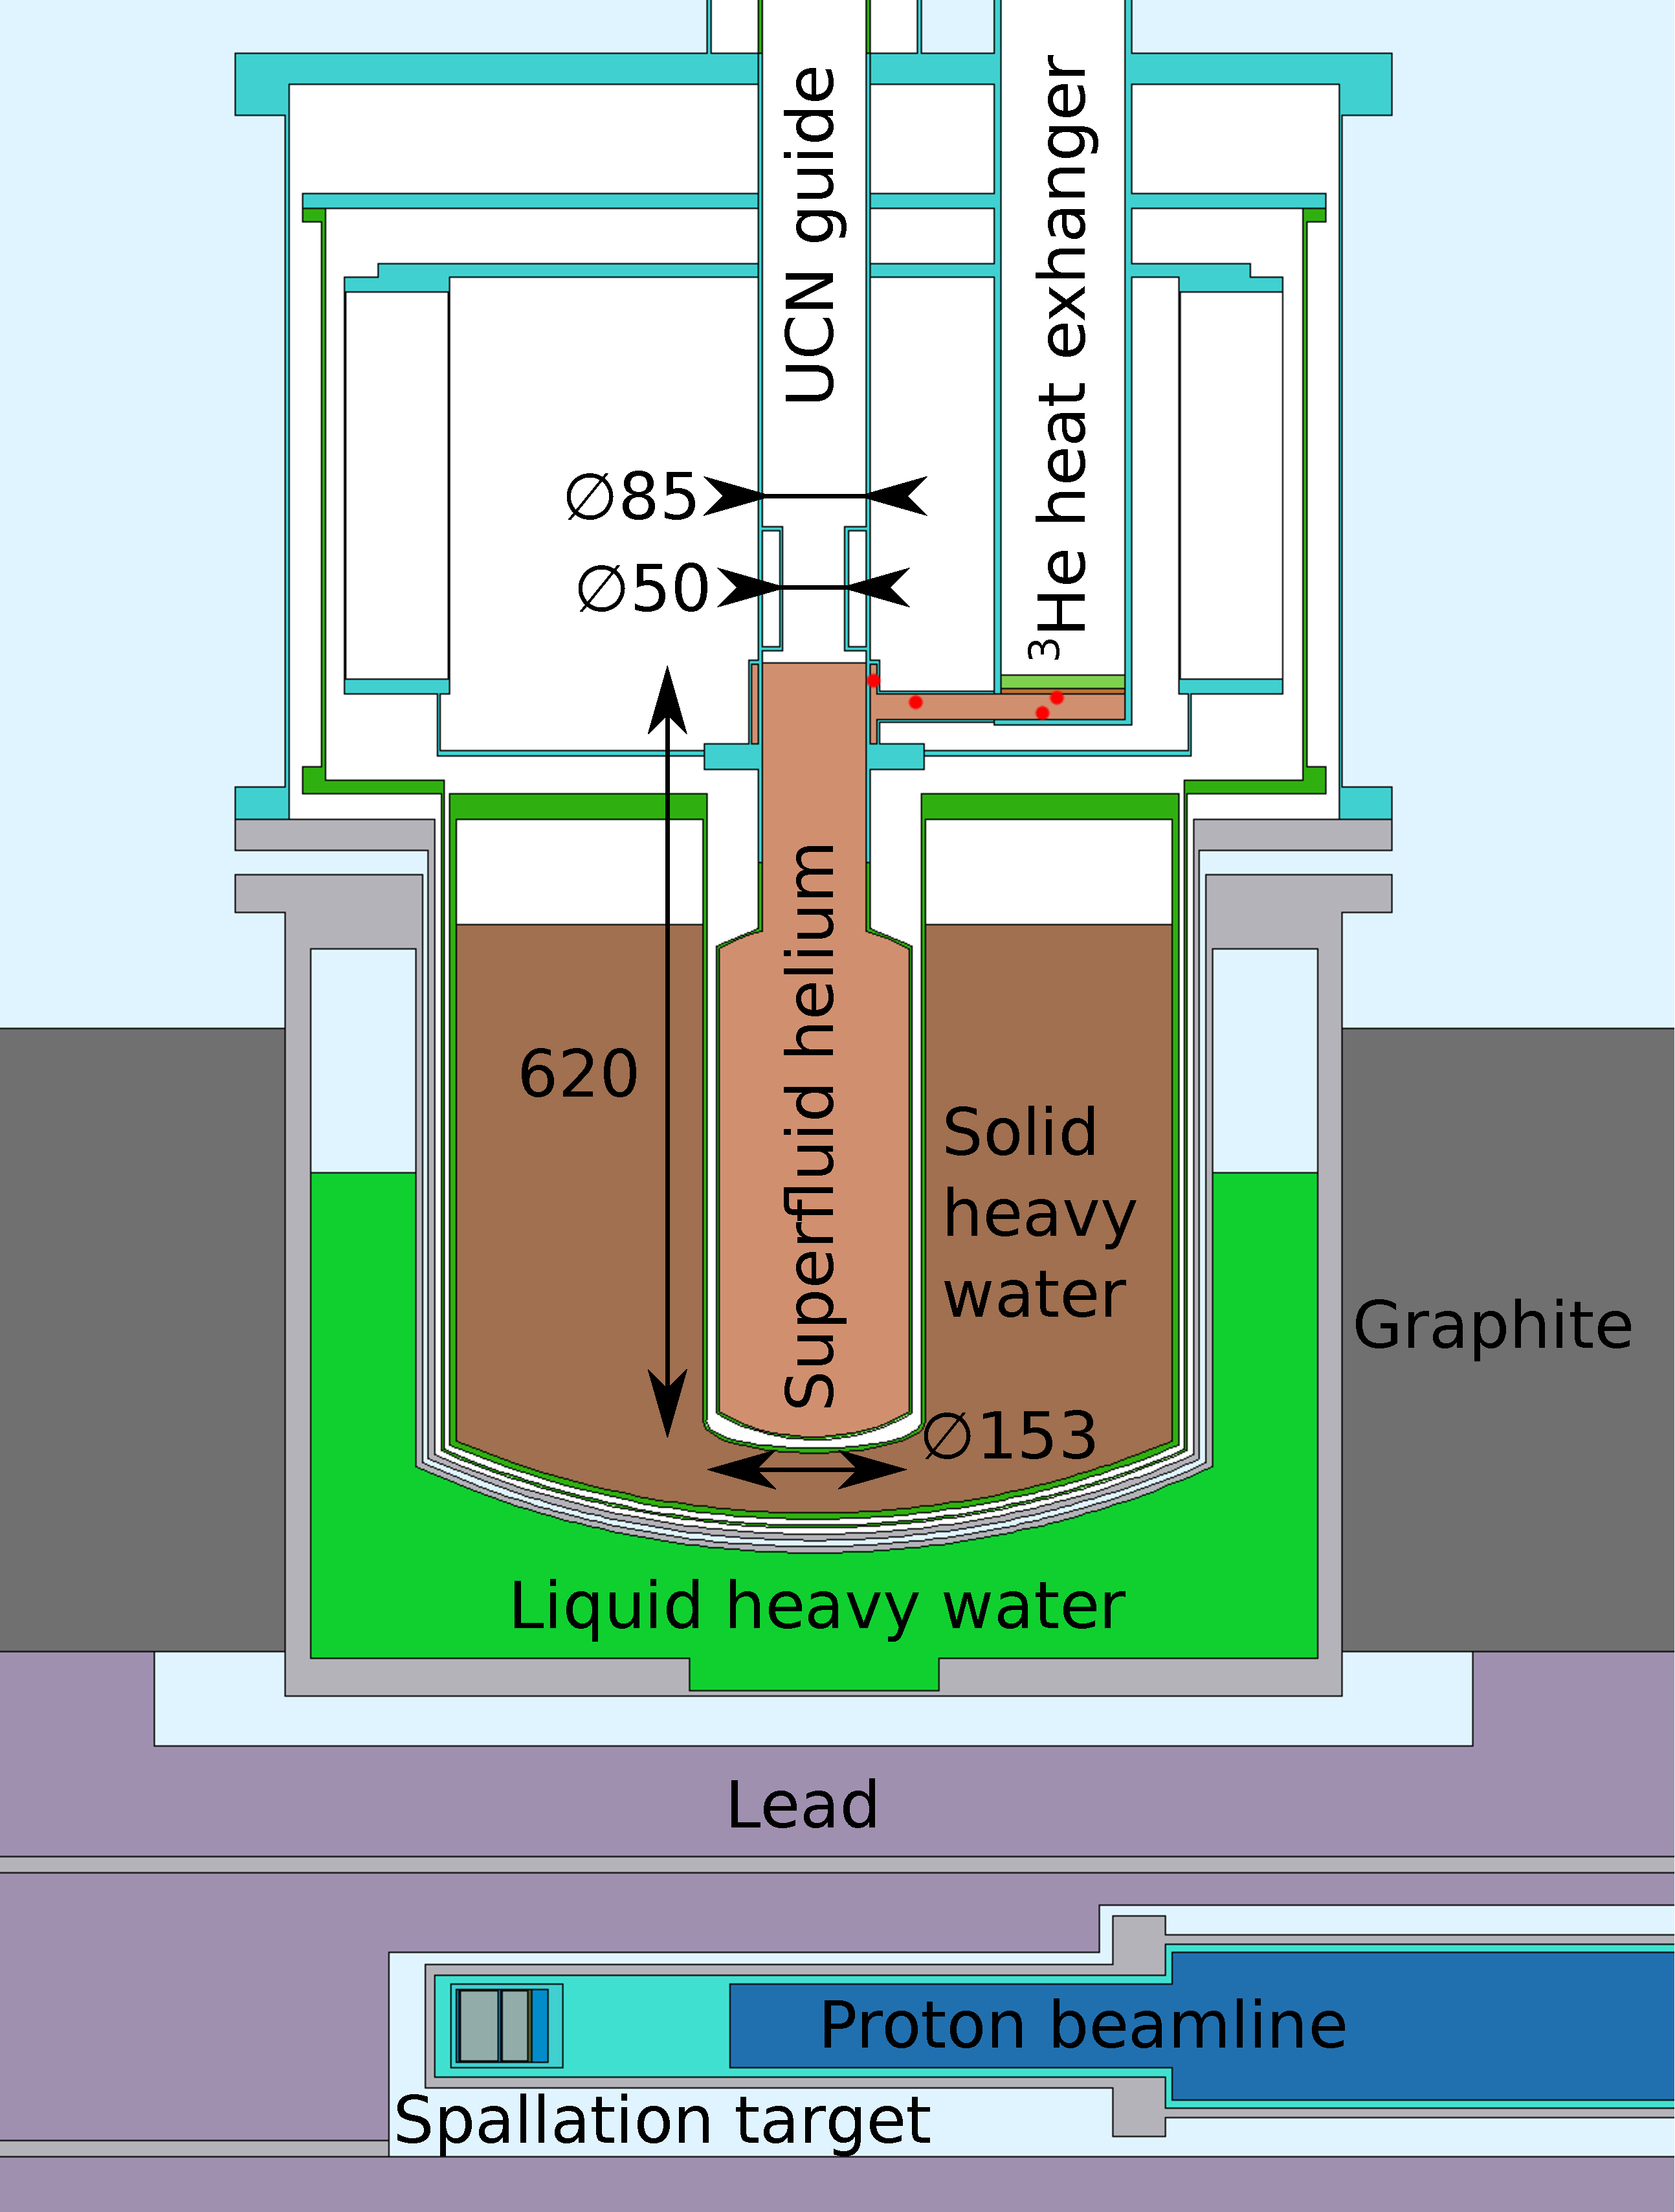
\includegraphics[width=0.6\textwidth]{MCNPmodel.pdf}
  \caption{MCNP model of the source. Red dots indicate the temperature
    sensors used to determine the temperature of the superfluid.}
  \label{fig:mcnpmodel}
\end{figure}


Fig.~\ref{fig:Counts_vs_temp_sim} and \ref{fig:storage_vs_temp_sim}
show the measured UCN counts and storage lifetime versus the
superfluid helium temperature for all four temperature sensors as well
as their simulations. To simulate the temperature of the superfluid
helium, different values for the imaginary Fermi potential $W$ were
taken into account as it is the needed parameter for the PENTrack
simulations. The UCN upscattering in the superfluid helium is
$\tau_{\mathrm{abs}}^{-1} = 2W/\hbar$~(see
Section~\ref{sec:ucnproperties}), and also
$\tau_{\mathrm{abs}}^{-1} = B T^7$. For two values of
$B$~($B = 0.016$/s and $B = 0.008$/s) at the desired temperature, the
imaginery fermi potential of superfluid helium can be calculated to
use in the simulations.


%{\bf{add how the temperature sensors are
%    simulated, what the tuned parameters were}}.

In these graphs, the filled circles represent the
measured data, and the emtpy squares and triangles represent the
simulations.  The empty squares are the simulations where the helium
vapour above the superfluid helium liquid is included, and empty
triangles are the simulations without the helium vapour. The
interpolations for the squares are shown in solid lines and the
interpolations for the emtpy triangles are shown with dotted and dashed
lines. The lines are only shown for readibility and are interpolation
of the simulated points.



\begin{figure}[h!]
  \centering
  \includegraphics[width=0.9\textwidth]{UCNCounts_vs_temp_ver3.pdf}
  \caption{Number of UCN extracted from the source at different
    superfluid helium temperatures after irradiating the target with
    1~$\mu$A proton beam current for 60~s(filled circles). The empty
    squares represent the simulations where the helium gas above the
    superfluid helium liquid is taken into account and the empty
    triangles represent the simulations where the helium gas is not
    included. The lines are interpolations of simulated data to guide
    the eye. The simulations were performed with two values of $B$:
    $B = 0.008$/s~(as shown with the top two lines) and
    $B = 0.016$/s~(as shown with the bottom two lines). The measured
    data is best matched with the simulations where $B = 0.016$/s
    where the helium gas is also taken into account.}
  \label{fig:Counts_vs_temp_sim}
\end{figure}

\begin{figure}[h!]
  \centering
  \includegraphics[width=0.9\textwidth]{StorageLifetime_vs_temp_ver3.pdf}
  \caption{Storage lifetime of UCN in the source at different
    superfluid helium temperatures~(filled circles).  The empty
    squares represent the simulations where the helium gas above the
    superfluid helium liquid is taken into account and the empty
    triangles represent the simulations where the helium gas is not
    included. The lines are interpolations of simulated data to guide
    the eye. The simulations were performed with two values of $B$:
    $B = 0.008$/s~(the top two lines and $B = 0.016$/s. The measured
    data is best matched with the simulations where $B = 0.016$/s
    where the helium gas is also taken into account.  The lines are
    interpolations of simulated data to guide the eye.}
  \label{fig:storage_vs_temp_sim}
\end{figure}

The simulations include two values for the upscattering paremeter $B$:
$B= 0.016$~s$^{-1}$, which represent the lower thick solid line~(empty
squares which represents the model where the helium vapour above the
superfluid helium liquid is included) and the dotted line~(empty
triangles where the helium vapour above the superfluid helium liquid
is not included), and $B= 0.008$~s$^{-1}$ which represent the solid
line~(empty squares) and the dashed line~(empty triangles). For the
simulations with $B= 0.016$~s$^{-1}$, when the helium vapour is also
included~(thick solid line), the measured data and simulations match
very well. Simulations without including the liquid vapour~(empty
traingles, dotted and dashed lines) show significant differences at higher liquid
temperatures. In this model, the storage lifetime and the UCN yield at
higher temperatures are overestimated. The reason for this is because
of the high upscattering rate of UCN in the helium vapour.



The helium vapour above the liquid is included in the simulations with
an upscattering rate
$\tau^{-1}_\mathrm{vapour} = \left< v \right> n \sigma_\mathrm{He,n}$
depending on the average atomic velocity $\left < v \right>$ which is
given by the vapour temperature, the vapour density $n$ given by the
saturated vapour pressure of the liquid and the vapour temperature,
and the thermal-neutron-scattering cross-section of helium
$\sigma_\mathrm{He,n} = 0.76~b$. This is because, the temperature of
the vapour right above the superfluid helium liquid is the same as the
superfluid temperature itself and it increases to room temperature
while moving along the guides. In this model, since the helium vapour
above the liquid has much higher temperature than the superfluid
helium liquid, the helium atoms have much higher velocities as
compared to the UCN. As a result, it might seem that the UCN are
stationary. Therefore, in the reference frame of the helium atoms,
thermal neutrons are moving towards the helium atoms.  It was assumed
that the vapour has the same temperature gradient as measured by
several temperature sensors on the outer guide wall. To include the
temperature gradient in the simulation, the guide volume was split
into 10~cm long sections and assigned each an averaged UCN
upscattering rate in that section.


%{\bf{I should prove that there is high upscattering rate of UCN in the
%    helium vapour. How is this calculated? Is it documented somewhere??}}.

\begin{figure}[h!]
  \centering
  \includegraphics[width=0.8\textwidth]{UCNrate_vs_temp_withsim_ver2.pdf}
  \caption{Histogram of measured UCN rates and temperatures from all
    four temperature sensors while the target is continuously
    irradiated with the UCN valve open. The emtpy squares represent
    the simulations where the helium gas above the superfluid helium
    liquid is taken into account and the empty tirangles represent the
    simulations where the helium gas above the superfluid helium
    liquid is not included.The lines are interpolations of simulated
    data to guide the eye. The simulations are performed for two
    values of $B$: $B = 0.016$/s~(shown by the two bottom lines), and
    $B = 0.008$/s~(shown by the top two lines). }
  \label{fig:rate_vs_temp_sim}
\end{figure}


The UCN rate in the steady-state mode of operation was measured at
different proton beam currents. When the proton beam current is above
1~$\mu$A, the temperature of the superfluid helium increases due to
the excess heat load. This causes the UCN rate to slowly decrease. The
overall result of those measurements and their simulations are shown
in Fig.~\ref{fig:rate_vs_temp_sim}. The empty squares represent the
simulations where the helium vapour above the superfluid helium liquid
is included in the simulations, and the empty triangles represent the
case where the helium vapour is excluded. The interpolation of the
simulations are shown in lines. The simulations are performed for two
values of parameter $B$: $B = 0.016$/s and $B = 0.008$/s. The
simulated data with a liquid helium upscattering parameter of
$B= 0.016$~s$^{-1}$~(thick solid line) slightly overestimates the drop
in the UCN rate with temperature. With $B= 0.008$~s$^{-1}$~(solid
line), it slightly overestimates the UCN rate, but better matches the
drop with temperature.

Unfortunately, the discrepancies between the temperature sensors in
the superfluid helium prevent a more accurate determination of the
upscattering parameter.

\section{Heater Test Versus Proton Beam Current}
One of the UCN experiments was designed to match the heater power from
the heaters wrapped around the UCN bottle with the proton beam
current. This type of measurements helps to understand the input heat
load on the cryostat.

The result of the heater tests were disscused in
Appendix~\ref{sec:heattest}. Applying heat to the superfluid helium
bottle gives rise to a temperature increase in the superfluid helium,
as well as a flow rate increase in the $^3$He pot. The amount of this
heat load is known simply by knowing the the applied current to the
heater tapes. However, the input heat load is not known in the case of
the target irradiation. As a result, the steady-state UCN yield were
measured at different proton beam currents as a way to calibrate the
proton beam current with the input current on the heaters. The target
irradiation at higher beam currents give rise to a temperature
increase in the superfluid helium. In addition, the increase in the
heat load increases the $^3$He flow rate in the $^3$He pot. The
comparison of the temperature and flow rate increase between these
experiments give an idea of the amount of applied heat load on the
superfluid helium bottle for each given proton beam current.

Even though the result of the data analysis for this experiment was
not conclusive, it gave an idea of the stability and the behaviour of
the helium cryostat, and a better experimental plan for the future.

Some unexpected anomalies were observed during the measurements. For
instance, when the 4~K resorvior was being filled, the flow rate in
the $^3$He pot as well as the temperature in the superfluid helium was
not stable. Another problem arose from the wait time between the
measurements. Before conducting a new measurement, it is essential to
wait long enough so that the superfluid helium temperature and $^3$He
flow rate get down to a stable value. In some cases, the wait time
between the measurements was not long enough, and therefore it was not
possible to assign a change in the superfluid helium temperature or
$^3$He flow rate. In addition, target irradiation should be long
enough so that the temperature and the $^3$He flow rate reach a stable
value.


\begin{figure}[h!]
  \centering 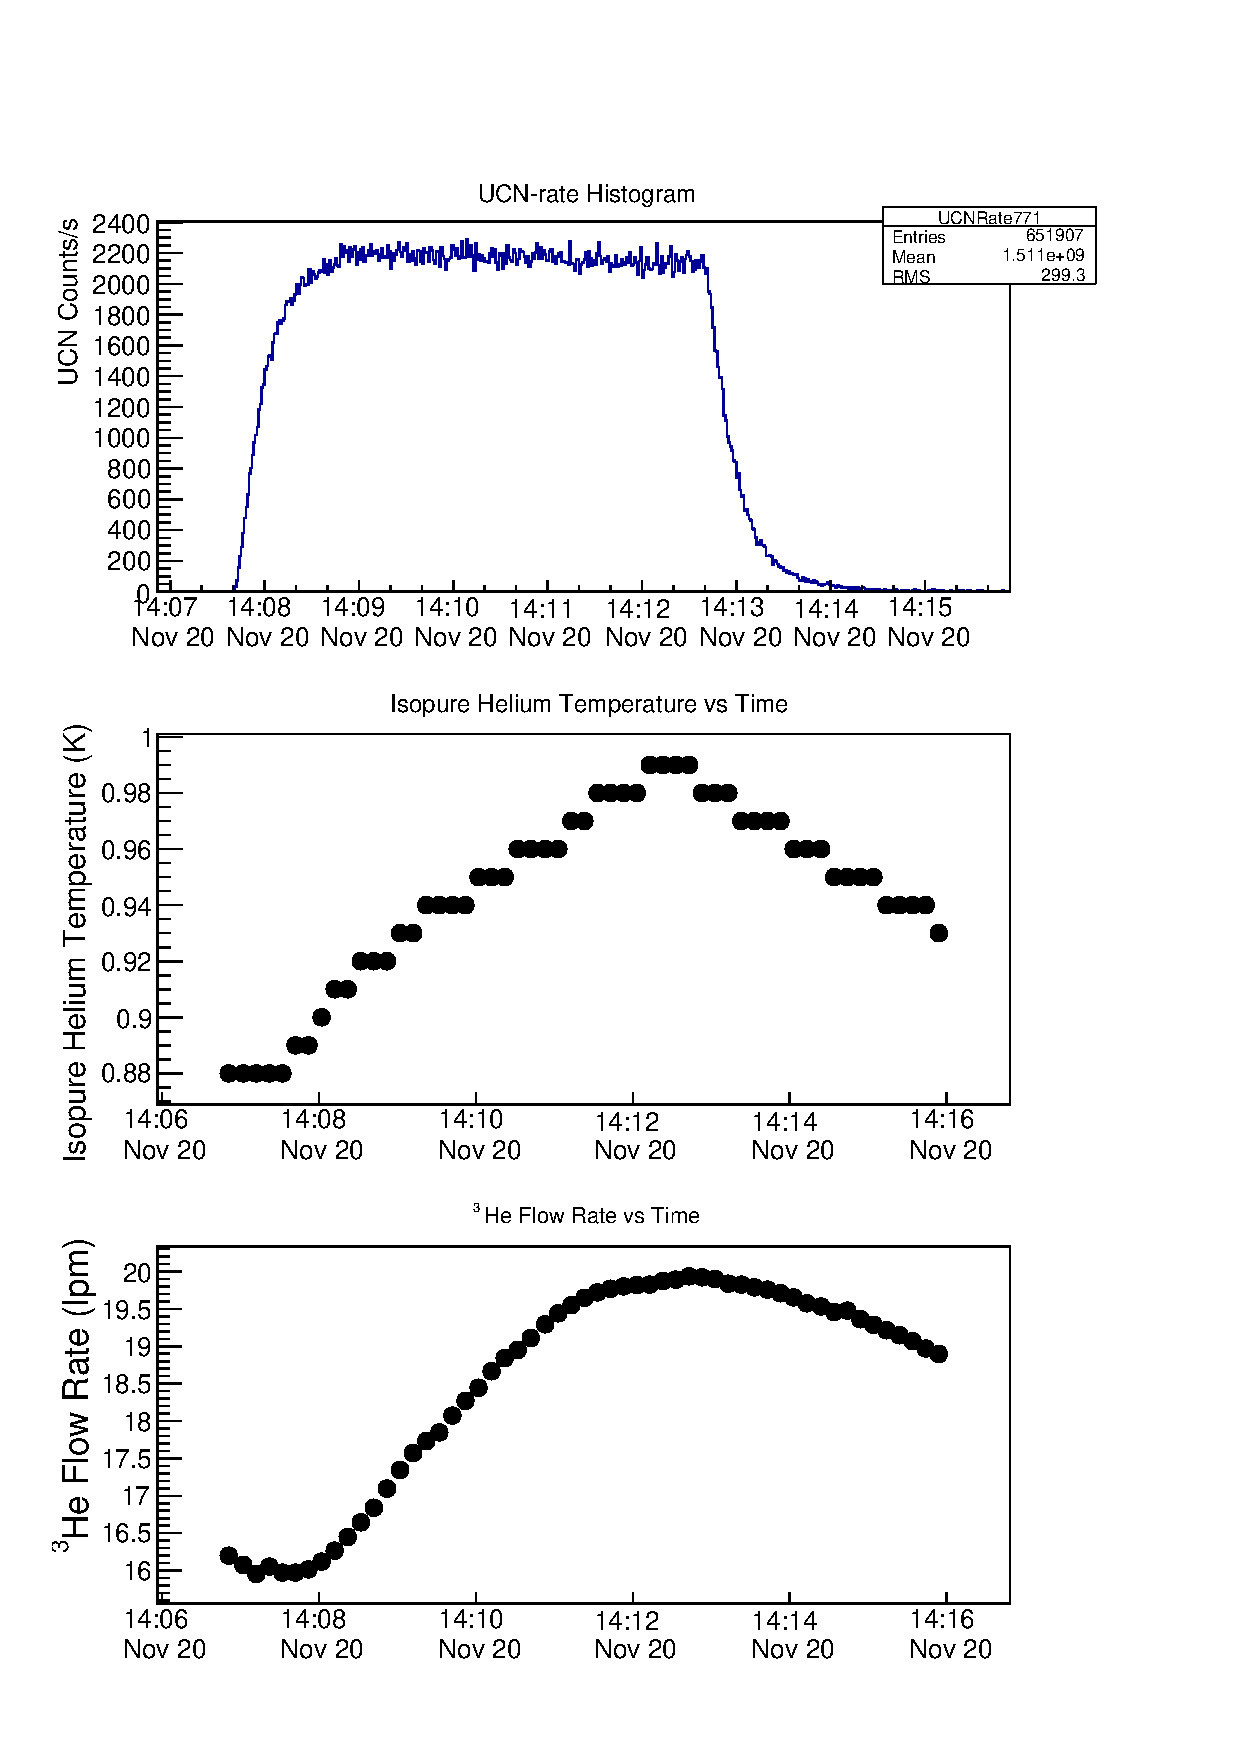
\includegraphics[width=0.8\textwidth]{problemrun.pdf}
  \caption{Steady-state UCN production data for 1.5~$\mu$A proton beam
    current. The top graph shows the UCN rate over time, the middle
    graph shows the superfluid helium temperature~(TS12) over time and
    the bottom graph shows the $^3$He flow rate versus time. Detail
    provided in text.}
\label{fig:problemrun}
\end{figure}

Fig.~\ref{fig:problemrun} shows an inconclusive run. The top graph
shows the UCN rate over time. This shows an increase in the UCN rate
after starting the target irradiation. At the end of the irraidation,
the UCN rate decays to the typical background rate. The middle graph
shows the temprature of the superfluid helium from the temprature
sensor TS12 over time. Here the irradiation of the target stopped
before the superfluid helium could reach a stable saturation
value. The bottom graph shows the flow rate in the $^3$He from sensor
FM1~(see Fig.~\ref{fig:gasflow} to see the position of the sensor). At
the beginning of the run, the flow rate was still going down, and it
did not reach a minimum stable value. Typically this value was around
14~SLM. In addition, the flow rate did not reach a maximum saturation
value due to short target irradiation time. Therefore, due to missing
informaion, the observed change in the $^3$He flow rate is not a good
measure of the input heat load on the cryostat and no result can be
concluded.


\section{Summary}
We successfully operated a superfluid-helium source for UCN at a
spallation source at TRIUMF. The result of the first UCN production
with this source at TRIUMF were discussed in this
chapter. The measurements include the UCN yield experiments, UCN
storage lifetime experiments, and steady-state UCN production
experiments as well as their simulations.

The maximum number of UCN achieved for the standard 1~$\mu$A proton
beam current at 60~s target irradiation time was 40,000, and the highest
number of UCN counts was 325,000 at 10~$\mu$A beam current and 60~s
target irradiation time. The experimental period took about two
weeks. In this time, the storage lifetime of UCN decreased from 37~s
to 27~s with about 2~\% decrease per day due to the source
contamination after opening the UCN valve. The UCN counts also showed
a decrease of about 40~\% due to the source contamination as well as
different experimental configuration at later dates. The steady-state
UCN rate showed to be around 1600~UCN/s/$\mu$A.

Although we were able to extract three times more UCN than ever before
due to the increased beam current on the spallation target, we
achieved only half of the previously best storage lifetime, mostly due
to the contamination of the source while it was moved, the burst dik
added to the UCN guide, and the new UCN valve not optimized for UCN
storage.

Simulations including the temperature-dependent up-scattering in
superfluid helium and helium vapour confirm that the former follows
$\tau_{\mathrm He} ^{-1} = B T^7$, matching the experimental UCN yield
and storage lifetime best with $B$ between 0.008/s and
0.016/s. Upscattering in helium vapour plays a significant role at
liquid temperatures above 1~K.

Future operation of this source will focus on better management of
contamination to increase the storage lifetime and on tests of new UCN
guides, valves, polarizers, and storage volumes.

This research provides the prerequisites for future developments: a
next-generation source with cooking power and UCN flux increased by
two orders of magnitude, and an experiment to measure the nEDM with a
sensitivity of $10^{-27}$~e$\cdot$cm. The excellent match of
simulations and experiment makes us confident that we can predict the
performance of this future source and experiment very well.


%To decrease the temperature of the superfluid by 0.1~K, a 5~min wait
%between the cycles is necessary. It is also concluded that, if
%interested in the $^3$He flow rate, the data acquisition should happen
%after the 4~K reservoir filling.



%\UCNreport{Detector Comparison\label{sec:detector_comparison}}
%Using the rotary valve

%\section{Background Measurements}
%With Ni foil

%\section{UCN guide Transmission Measurements}

%\section{Result And Conclusion}

%\begin{description}
%\item{I think this belongs to this chapter: UCN production by
%  multiphonon excitation in superfluid helium (I can use my candidacy
%  report for this part as a start)}
  
%\item{Some information about the detector}
  
%\item{UCN data goes here}
  
%\item{what else?}
%\end{description}
